\chapter{GLADE+ Bright Galaxies as Redshift Tracers}
\label{chap:methodology}

%The core idea investigated in this thesis is the use of \textbf{bright galaxies} as redshift tracers for \ac{GW} events. The \texttt{GLADE+} galaxy catalog is a comprehensive database of galaxies in the local Universe, but it suffers from incompleteness at high redshifts. This incompleteness arises from the limited depth of the catalog, which is primarily designed to cover the local Universe, owing to the sensitivity constraints of the current \ac{EM} telescope. We overcome this limitation by focusing on the brightest galaxies in the catalog, which are more likely to be well-represented and can provide a more accurate estimate of the redshift of \ac{GW} events. This essentiaally makes the catalog deeper and more complete at high redshifts, while allowing us to use the \texttt{GLADE+} catalog as a proxy for the underlying matter distribution in the Universe.
The core idea investigated in this thesis is the use of \textbf{bright galaxies} as redshift tracers for \ac{GW} events. The \texttt{GLADE+} galaxy catalog is a comprehensive compilation of galaxies in the local Universe, designed primarily to support multi-messenger follow-up observations. However, it suffers from incompleteness at higher redshifts due to the limited sensitivity of current \ac{EM} surveys.

To mitigate this limitation, we focus on the brightest galaxies in the catalog, which are more likely to be detected at higher redshifts and better trace the large-scale structure. By applying a brightness-based pruning strategy, we effectively enhance the redshift reach and completeness of the catalog, allowing \texttt{GLADE+} to serve as a more accurate proxy for the underlying matter distribution relevant to dark siren cosmology.

The results and methodology developed in this thesis have been submitted for peer review to the \textit{\ac{MNRAS}} and are available as a preprint on \texttt{arXiv}~\citep{naveed2025dark}, contributing to the growing body of research in \ac{GW} cosmology.

\section{Bright Galaxy Subsets}
The analysis begins with the construction of \textbf{bright galaxy subsets}, denoted \texttt{GLADEPXX}, where only the top $XX\%$ of galaxies by cumulative $K$-band luminosity are included. The $K$-band luminosity is chosen as it is better associated with the mass of the galaxies \citep{strazzullo2006near,sureshkumar2021galaxy}. Limiting the analysis to these bright subsets allows us to:
\vspace{-1em}
\begin{itemize}
  \item Reduce the out-of-catalog correction by focusing on bright galaxies likely to be well-represented.
  \vspace{-1em}
  \item Improve the signal-to-noise ratio of the statistical redshift prior.
  \vspace{-1em}
  \item Minimize the inclusion of poorly characterized or faint galaxies.
\end{itemize}

The bright galaxy subsets are defined by selecting galaxies based on their absolute magnitude, which is inferred from their redshift and apparent magnitude. For a given subset, the dimmest galaxy sets the absolute magnitude limit, $M_{\mathrm{max}}$, for that subset. This limit is then used in the Schechter luminosity function to adjust the out-of-catalog contribution, effectively reducing its impact. By focusing on the brightest galaxies, we assume that they trace the mass distribution in the Universe more effectively, and are more likely to host \ac{CBC} events.

This approach improves the completeness of the galaxy catalog in the high-redshift regime, as the out-of-catalog contribution becomes smaller. Figure~\ref{fig:z_dist} illustrates how the redshift distribution shift towards higher values making the catalog more complete, highlighting the effectiveness of this method in probing deeper $z$--ranges.

\begin{figure}[h!]
  \centering
  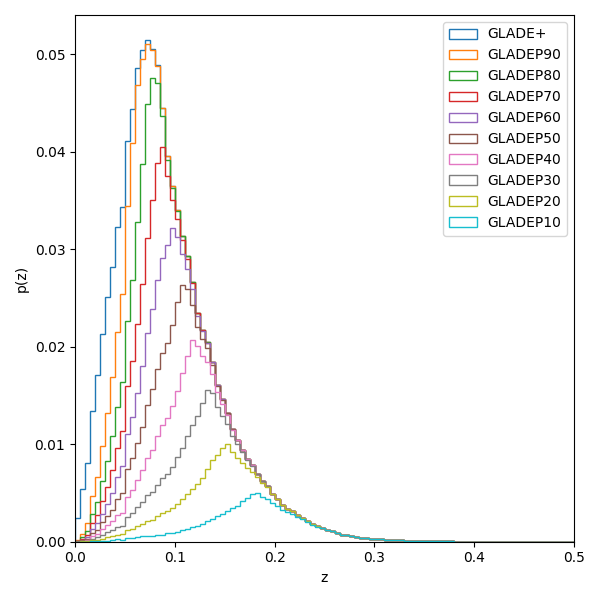
\includegraphics[width=0.7\linewidth]{figures/z_dist_perc.png}
  \caption[Normalized redshift distributions $p(z)$ for the \texttt{GLADE+} galaxy catalogue and its brightest percentiles.]{Normalized redshift distributions $p(z)$ for the full \texttt{GLADE+} galaxy catalogue (blue) and the brightest percentiles (other curves). Each subset, labeled \texttt{GLADEPXX}, includes only the top XX\% brightest galaxies in the $K$-band. Focusing on increasingly brighter subsets shifts and sharpens the redshift distribution, effectively probing deeper ranges in $z$.}
  \label{fig:z_dist}
\end{figure}

\subsection{Trade-Offs and Limitations}

While bright subsets reduce catalog incompleteness, they may inadvertently exclude genuine host galaxies, especially if those lie in less luminous systems or in underrepresented regions of the catalog. The effectiveness of these cuts depends on the intrinsic distribution of host galaxies, the depth and completeness of the original catalog, and the accuracy of $K$-band photometry. 
%The effectiveness of these cuts therefore depends on:
%\vspace{-1em}
%\begin{itemize}
%  \item The depth and completeness of the original catalog.
%  \vspace{-1em}
%  \item The intrinsic distribution of host galaxies.
%  \vspace{-1em}
%  \item The accuracy of $K$-band photometry.
%\end{itemize}

One major limitation of this approach is that brightest galaxies may not be representative of the overall galaxy population, as they may be biased towards certain types of galaxies or regions of the sky. This effect is however mitigated by the fact that we are using the $K$-band luminosities, which are good tracer for the stellar mass \citep{strazzullo2006near,sureshkumar2021galaxy}, and in turn the overall matter distribution. Furthermore, the bright galaxy subsets are constructed from the \texttt{GLADE+} catalog, which is designed to be a complete and representative sample of galaxies in the local Universe. This means that the bright galaxy subsets are likely to be representative of the overall galaxy population, and give a crude estimate of the matter distribution, even if they are not a complete sample.

Estimating the true redshift of a \ac{GW} event by the nearest brightest galaxies is supposed to have a negligible effect on the results. This is because the bright galaxies are more likely to be located in regions of high density, such as galaxy clusters or groups, which are also likely to host \ac{GW} events. This means that the bright galaxies are likely to be located in the same large-scale structure as the \ac{GW} event, and thus provide a good estimate of the redshift of the event. 

One important thing to note is that while the use of a bright subset enhances the completeness of the catalogue at high redshifts, it also introduces a trade-off. If the brightness cut is too restrictive, the exclusion of galaxies may lead to a loss of information and in turn an underrepresentation of the overall matter distribution, potentially biasing the results. One needs to carefully balance these considerations by comparing different brightness thresholds. A moderate brightness cut will maximize the benefit in terms of depth without incurring significant bias. The appropriate brightness cut can be established only via a set of astrophysics-motivated large-scale simulations. A \ac{GW} \textit{\ac{MDC}}, detailed in the next chapter, using the simulated \texttt{BUZZARD} galaxy catalog from the \ac{DES} Collaboration~\citep{DES:2019jmj,DES:2021bwg}.  
%It is designed to determine the optimal brightness threshold which maximizes the measurement precision with bright subsets while keeping the biases in control. Tests performed in the process will help refine the methodology and ensure that the improved constraints on the Hubble constant are robust against additional systematic uncertainties.

Another thing to note is that due to to the brightness cut, we may lose the low-redshift galaxies, in turn losing information in the nearby Universe. This can be easily overcome in the future by combining the use a complete galaxy catalog in the nearby Universe, with the bright galaxy subsets in the high-redshift regime. Such an approach would not only allow us to have a complete galaxy catalog in the nearby Universe, but also probe deeper redshifts using bright galaxies while reducing the out-of-catalog correction. However, this is not a trivial task, as it requires a smooth and consistent transition between the two regimes. But nonetheless, this is a good first step towards improving the completeness of the galaxy catalog and future work could further refine this approach by using different redshift tracers in different redshift regimes, such as using the bright galaxy subsets in the high-redshift regime, and a complete galaxy catalog in the nearby Universe.

While the bright galaxy subsets may not be a perfect representation of the overall galaxy population, they are still a useful tool for improving the completeness of the galaxy catalog and reducing the out-of-catalog correction. The error incurred by using the bright galaxies as redshift tracers may be small compared to the current errors in luminosity distance measurements from the \ac{GW} events, this may become a problem in the future as the \ac{GW} measurements become more precise. In this case, one may need to use more sophisticated methods to estimate the redshift of the \ac{GW} event, such as more complex models of the galaxy population, but for now this is a good first step towards improving the completeness of the galaxy catalog and reducing the out-of-catalog correction, by leveraging the currently available \ac{EM} data.

%In Chapters~\ref{chap:results} and~\ref{chap:mockdata}, we quantify these trade-offs using both real data and mock catalogs.

\begin{figure}[h!]
  \centering
  \begin{subfigure}{0.32\textwidth}
    \includegraphics[width=\linewidth]{figures/test_frame_g_0.png}
    \label{fig:gladep100}
  \end{subfigure}
  \begin{subfigure}{0.32\textwidth}
    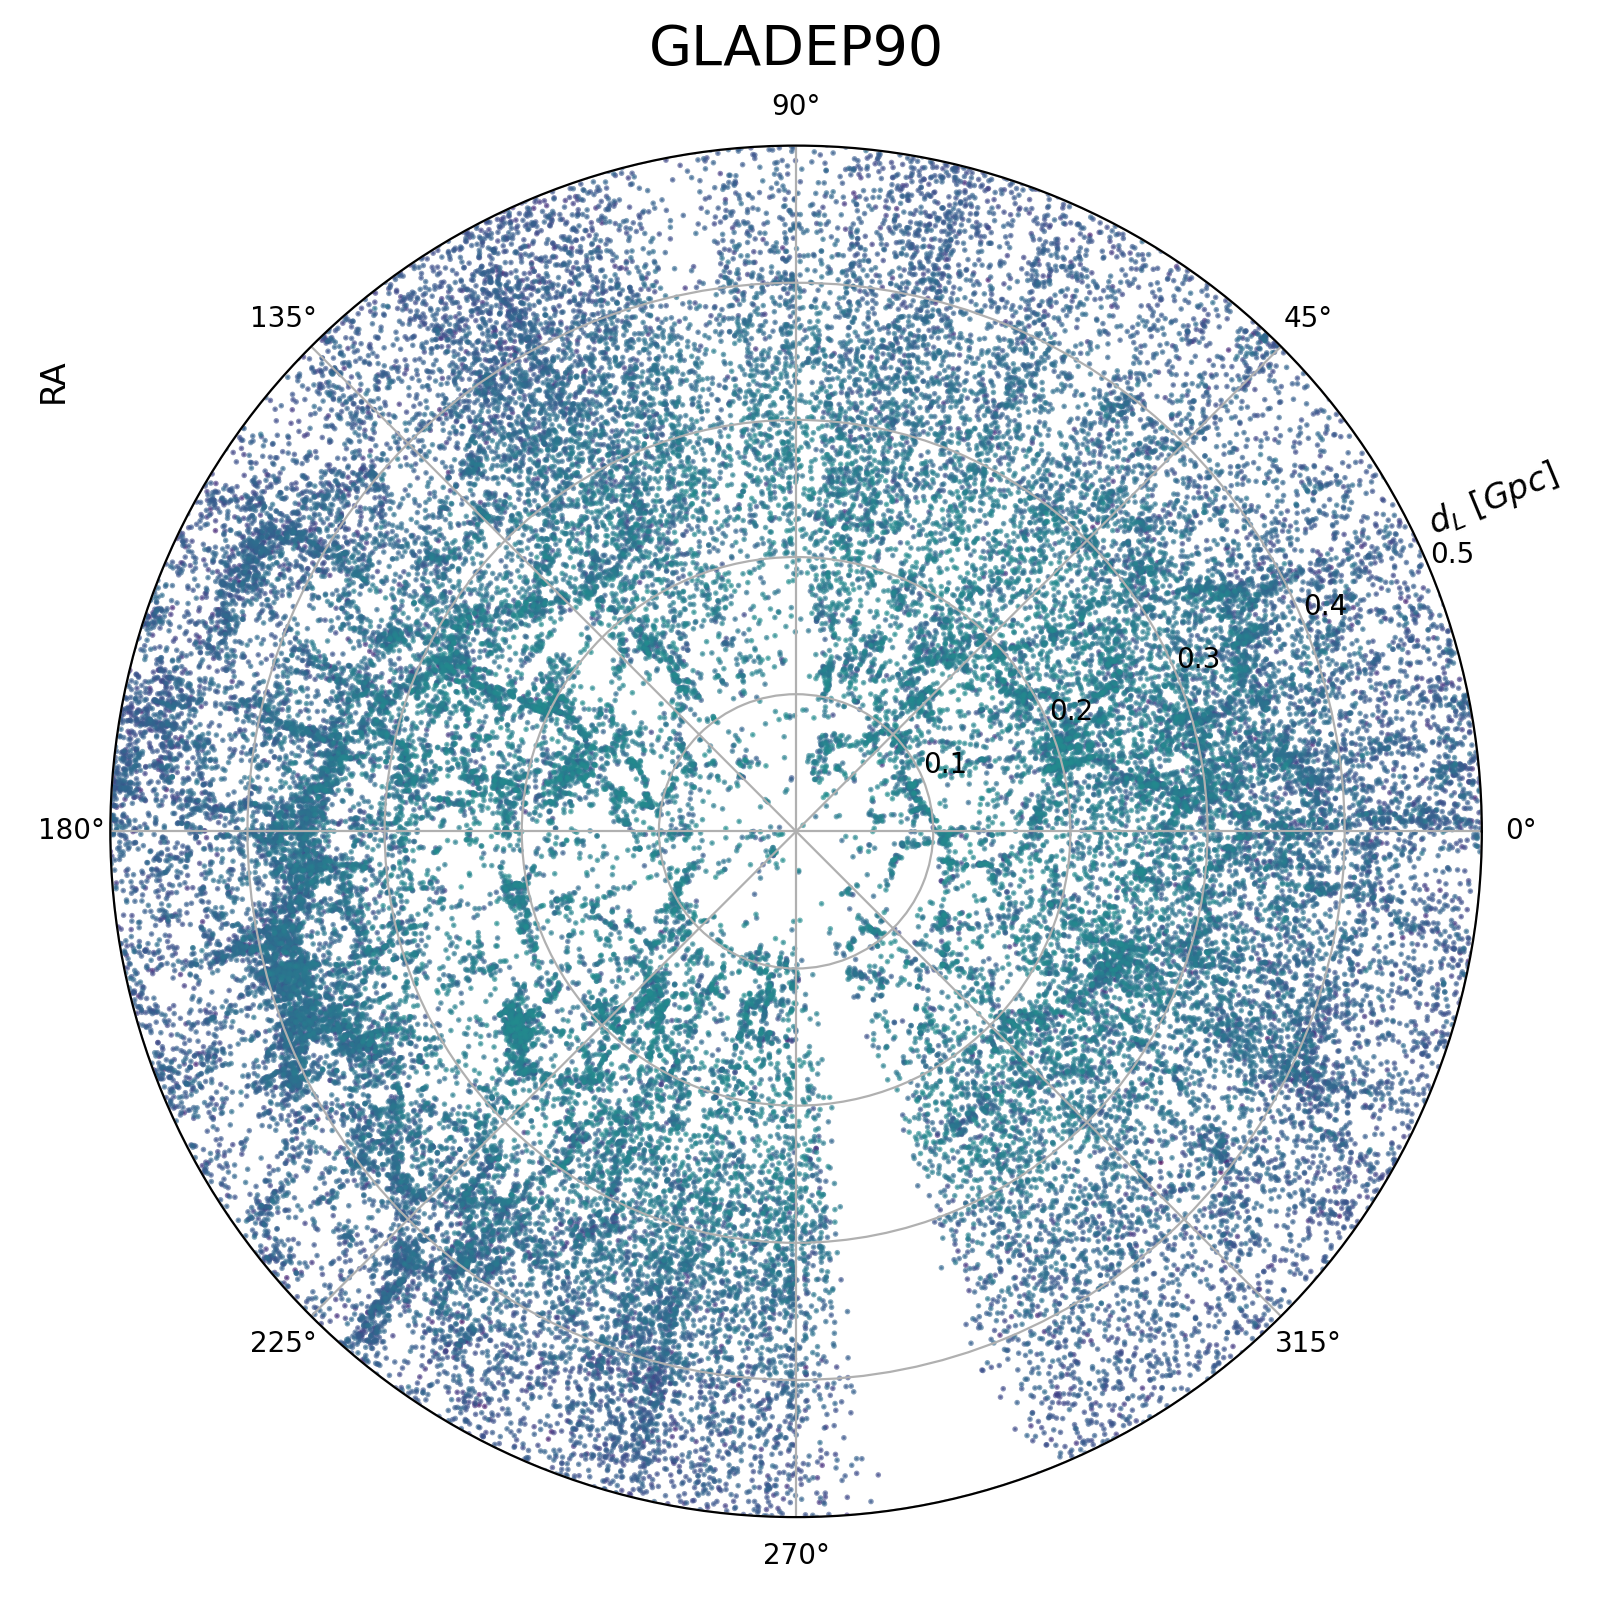
\includegraphics[width=\linewidth]{figures/test_frame_g_1.png}
    \label{fig:gladep90}
  \end{subfigure}
  \begin{subfigure}{0.32\textwidth}
    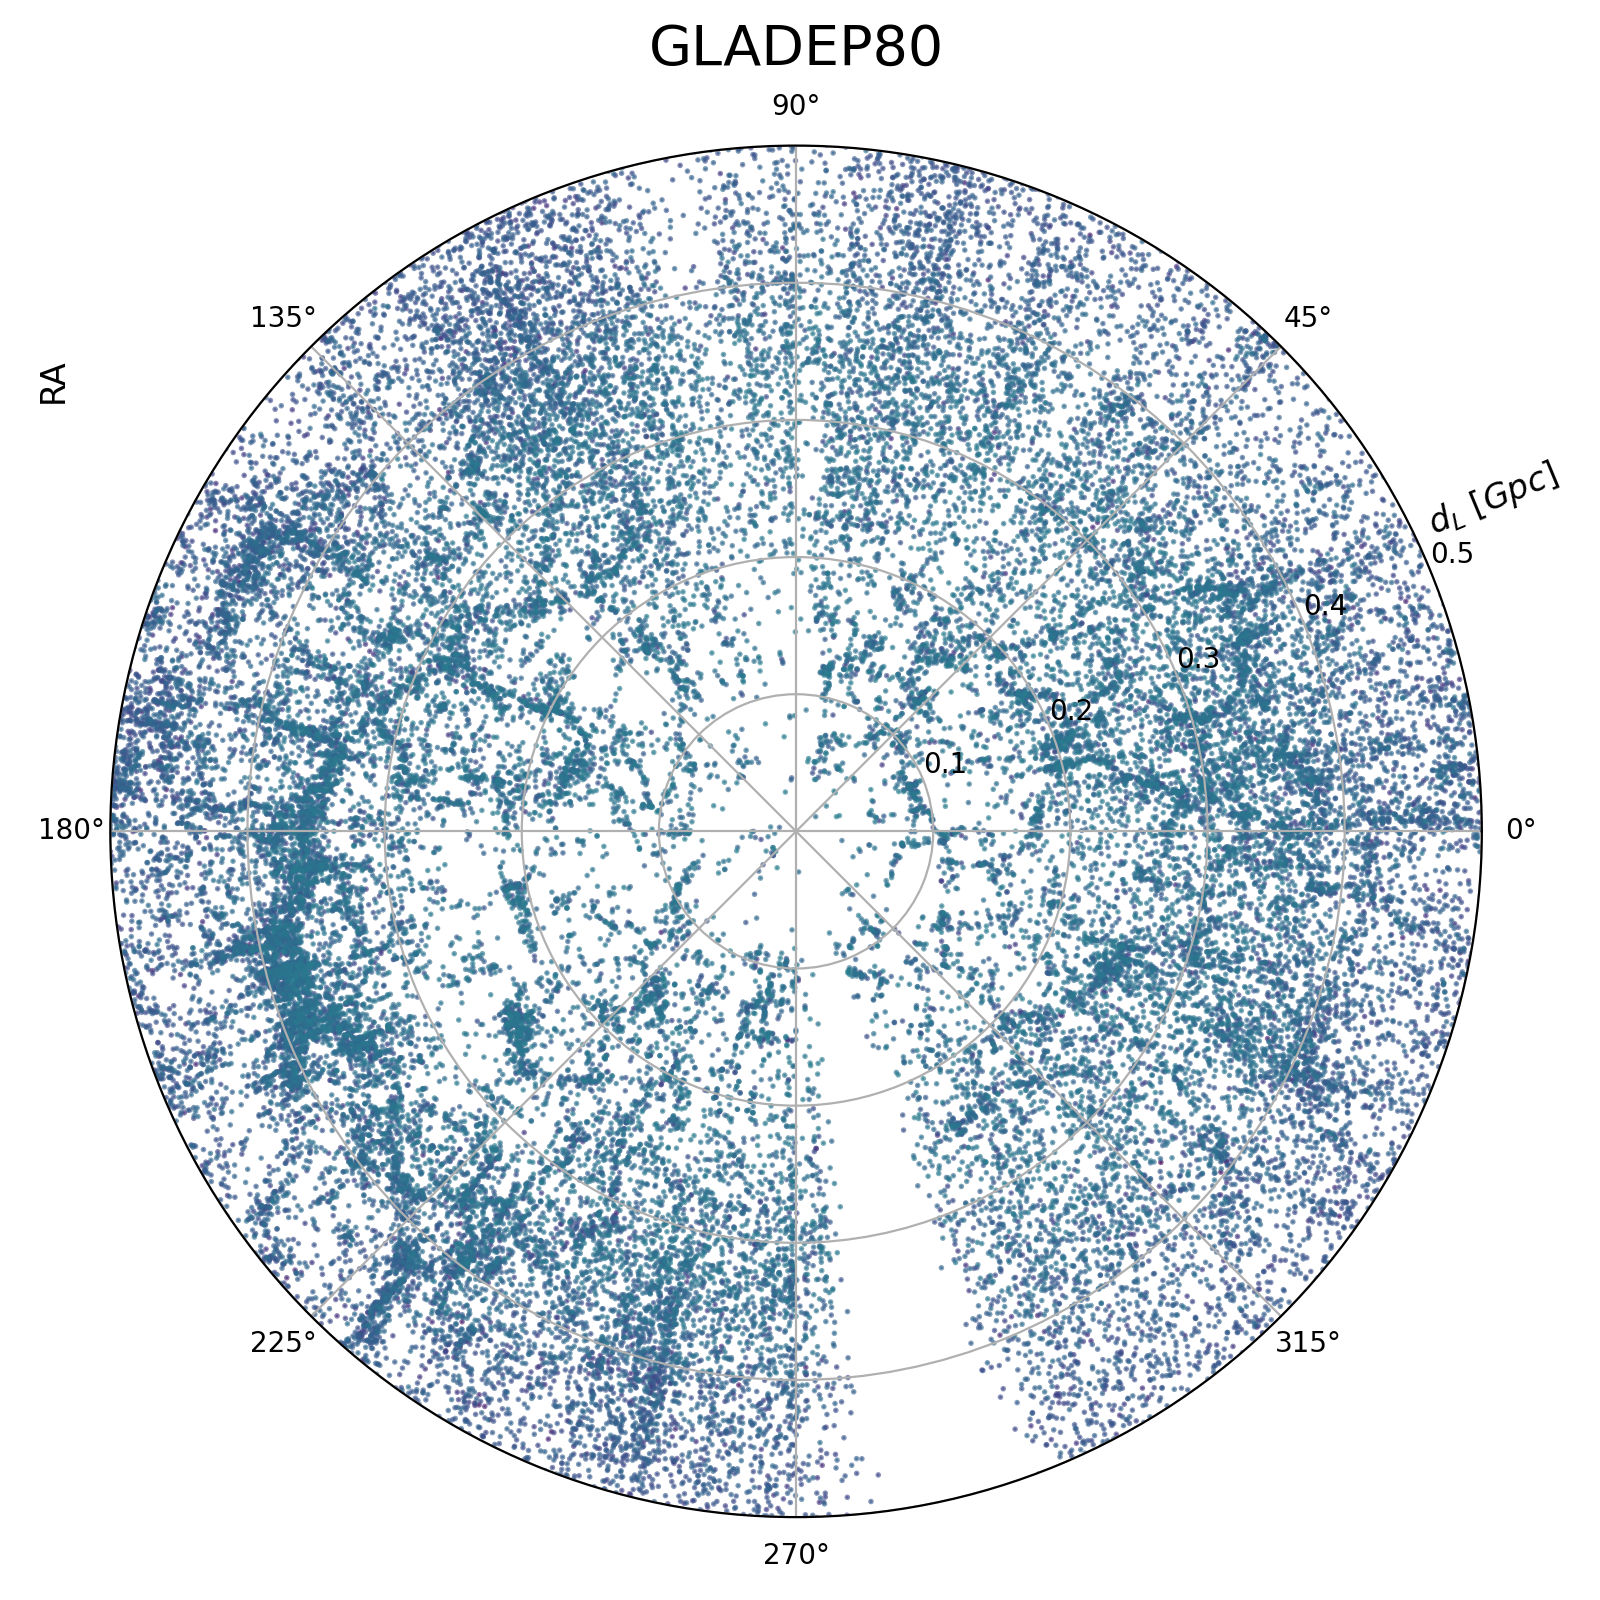
\includegraphics[width=\linewidth]{figures/test_frame_g_2.png}
    \label{fig:gladep80}
  \end{subfigure}
  \vspace{0.5em}
  \begin{subfigure}{0.32\textwidth}
    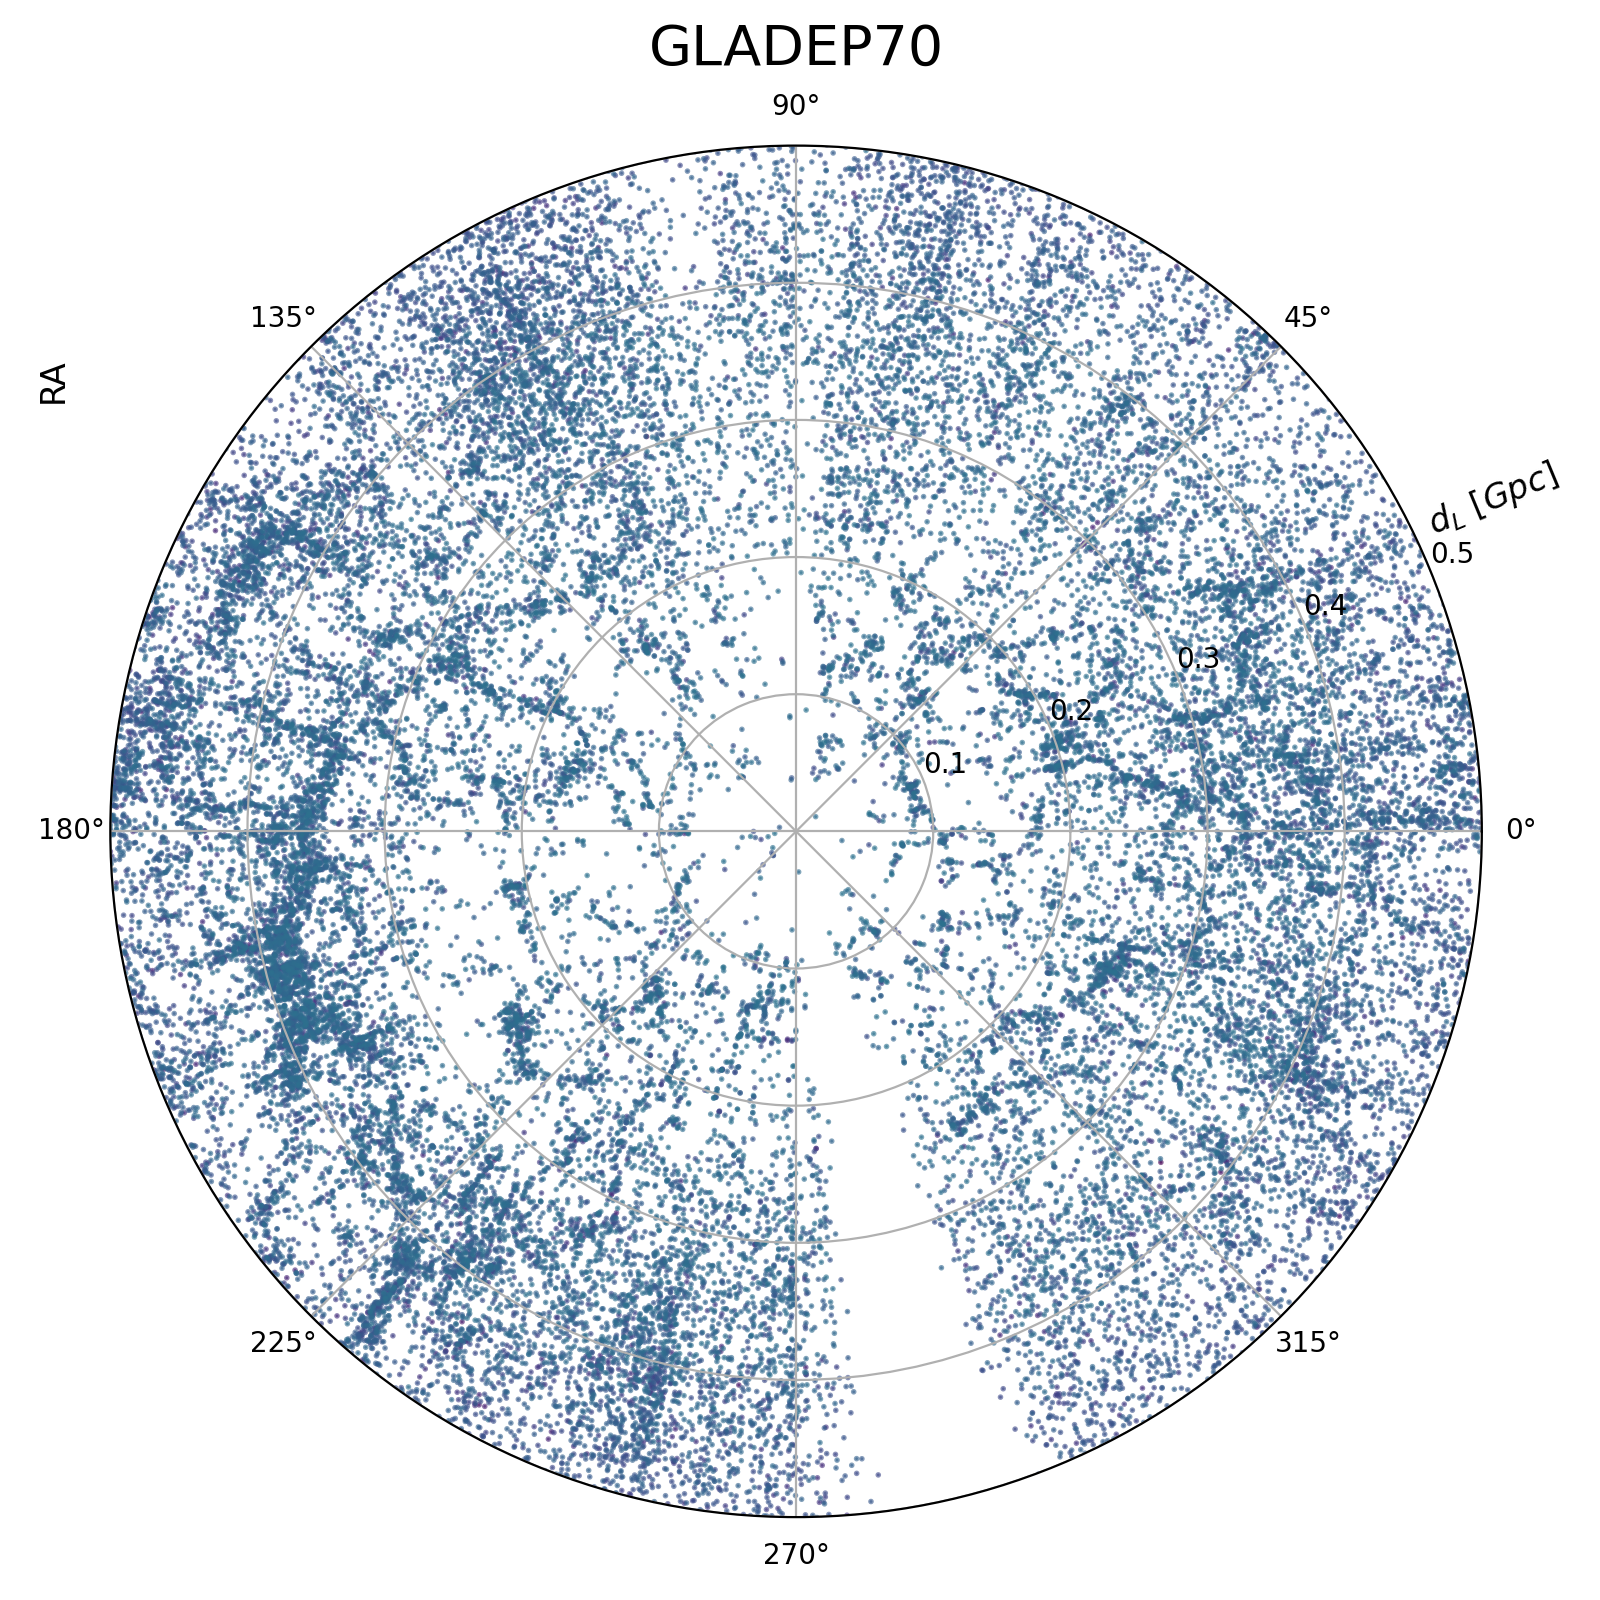
\includegraphics[width=\linewidth]{figures/test_frame_g_3.png}
    \label{fig:gladep70}
  \end{subfigure}
  \begin{subfigure}{0.32\textwidth}
    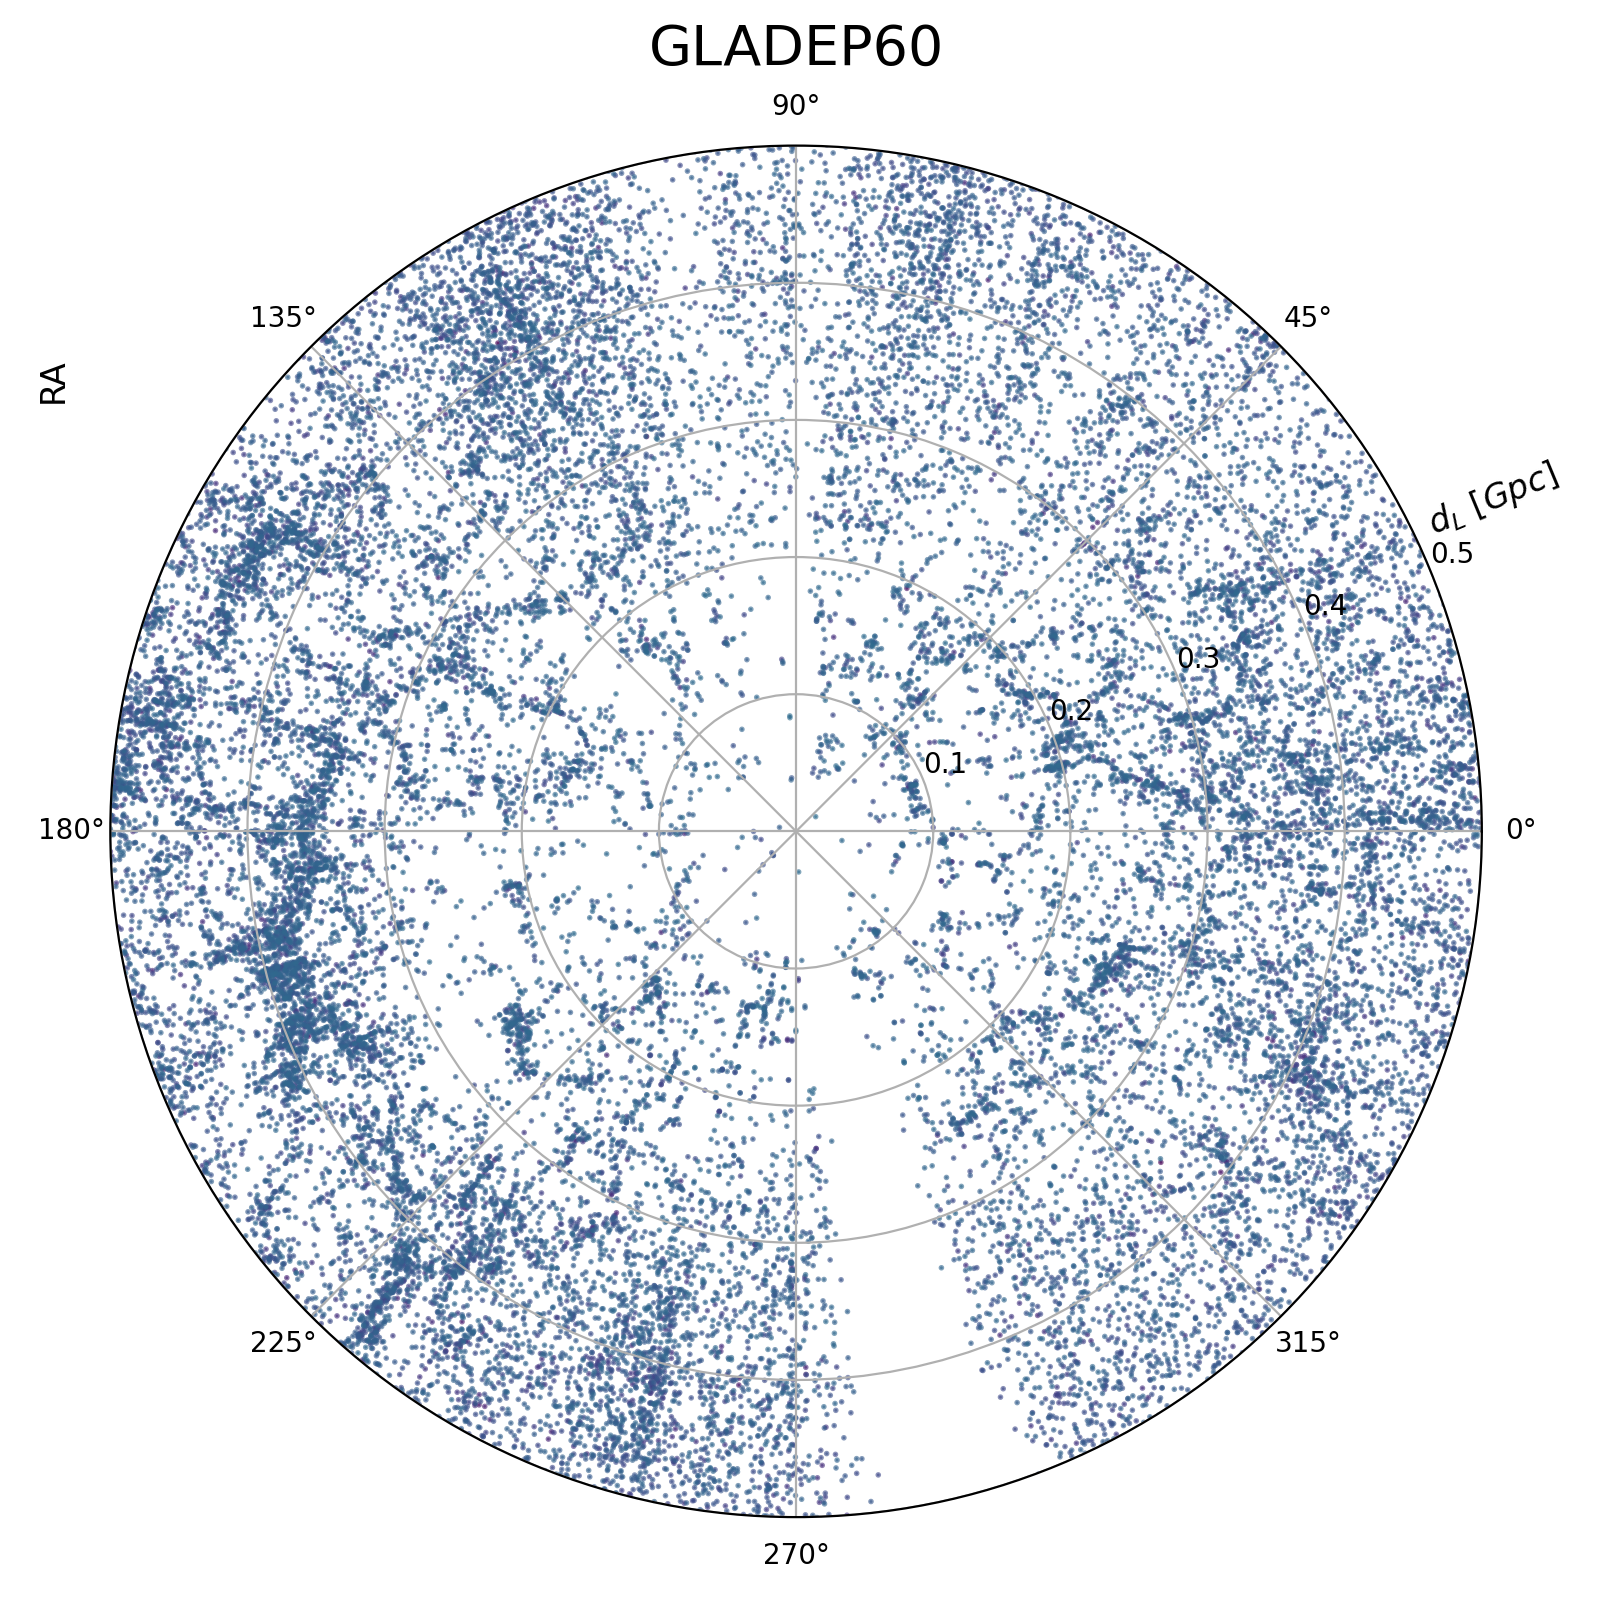
\includegraphics[width=\linewidth]{figures/test_frame_g_4.png}
    \label{fig:gladep60}
  \end{subfigure}
  \begin{subfigure}{0.32\textwidth}
    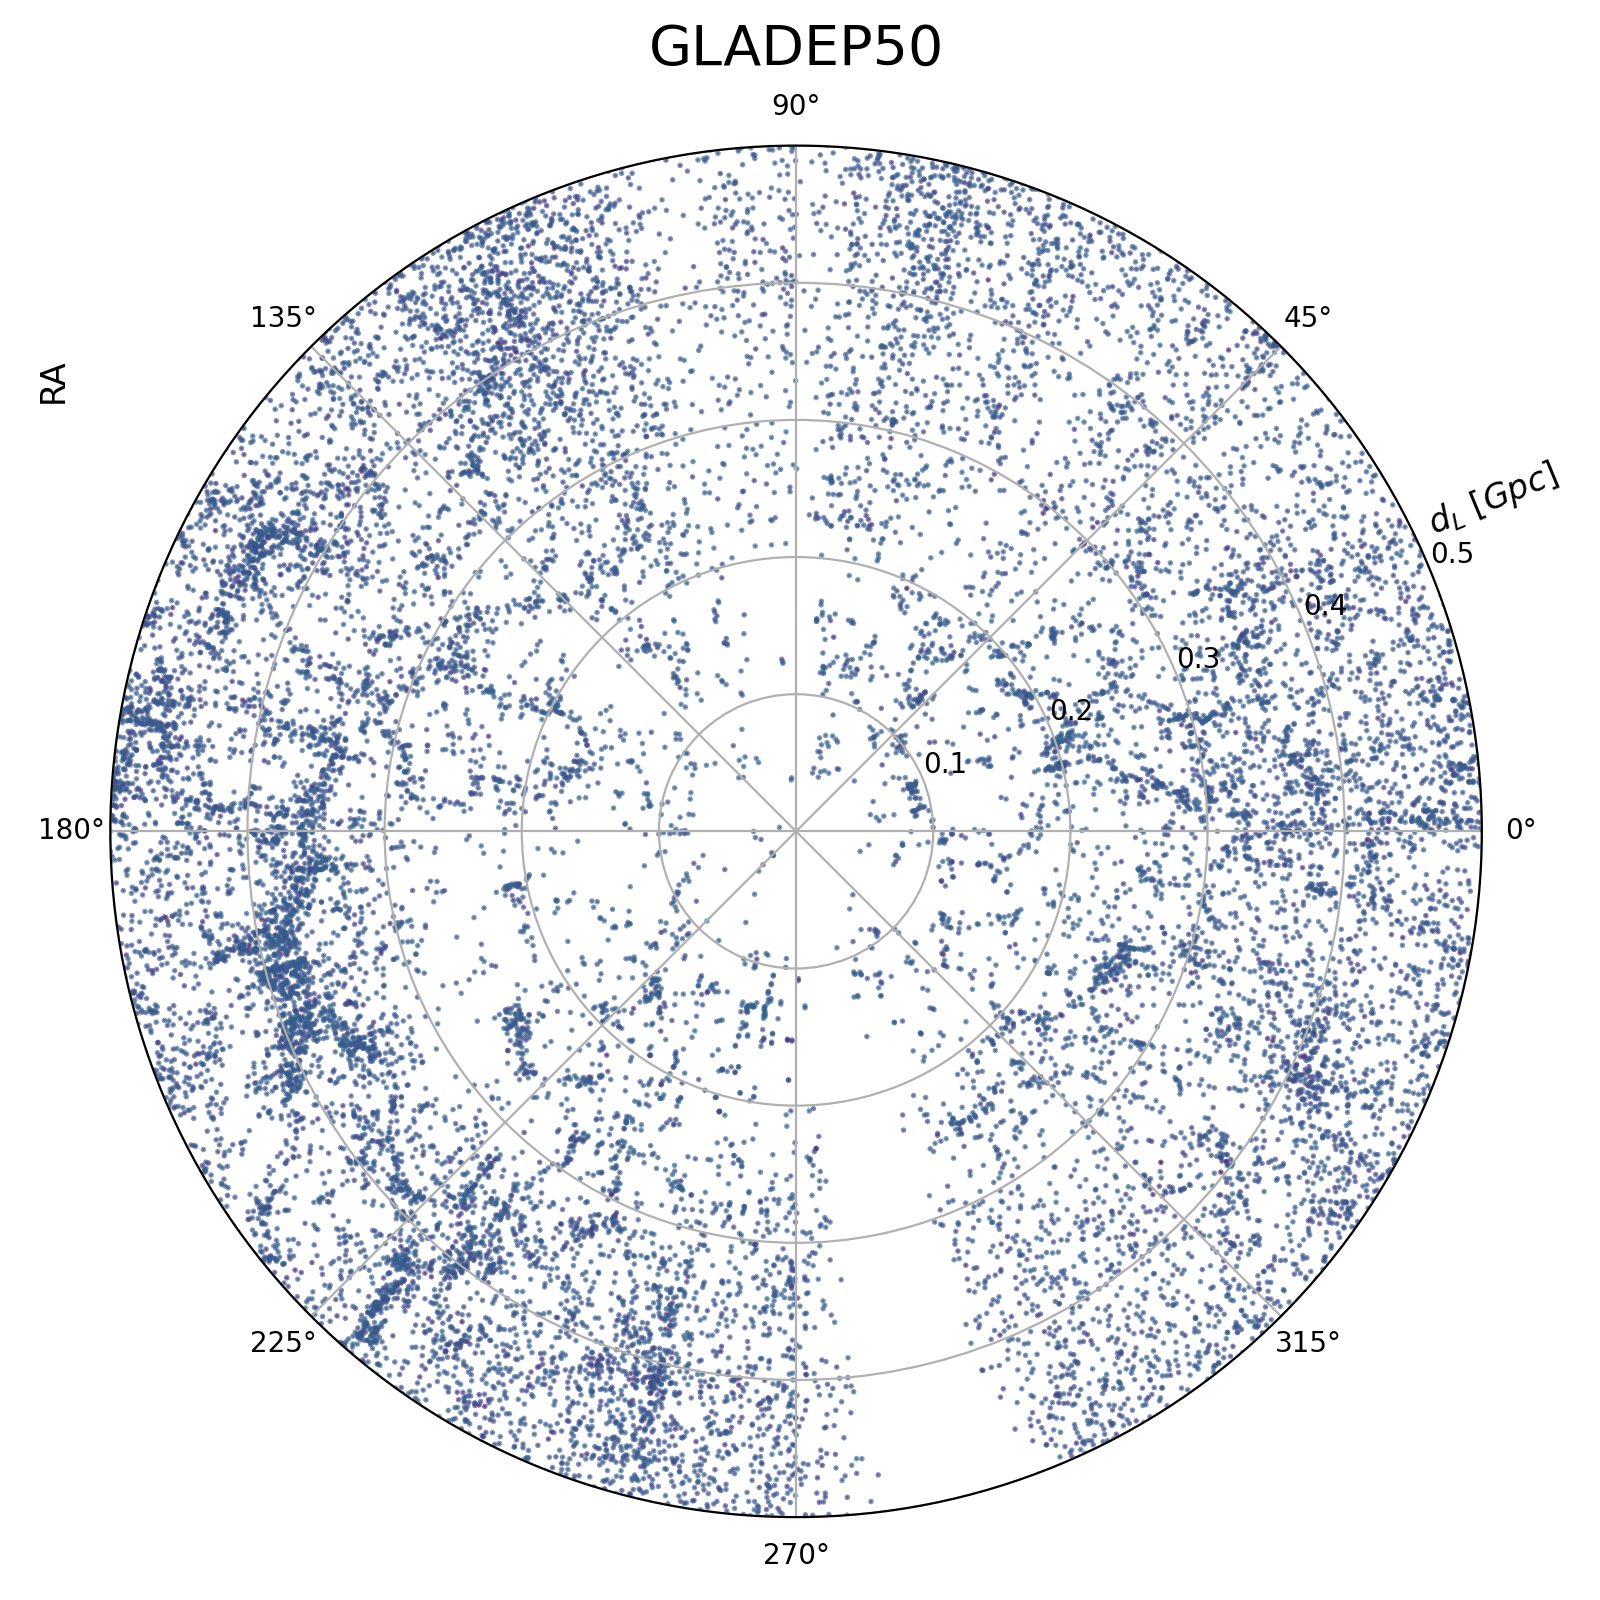
\includegraphics[width=\linewidth]{figures/test_frame_g_5.png}
    \label{fig:gladep50}
  \end{subfigure}
  \vspace{0.5em}
  \begin{subfigure}{0.32\textwidth}
    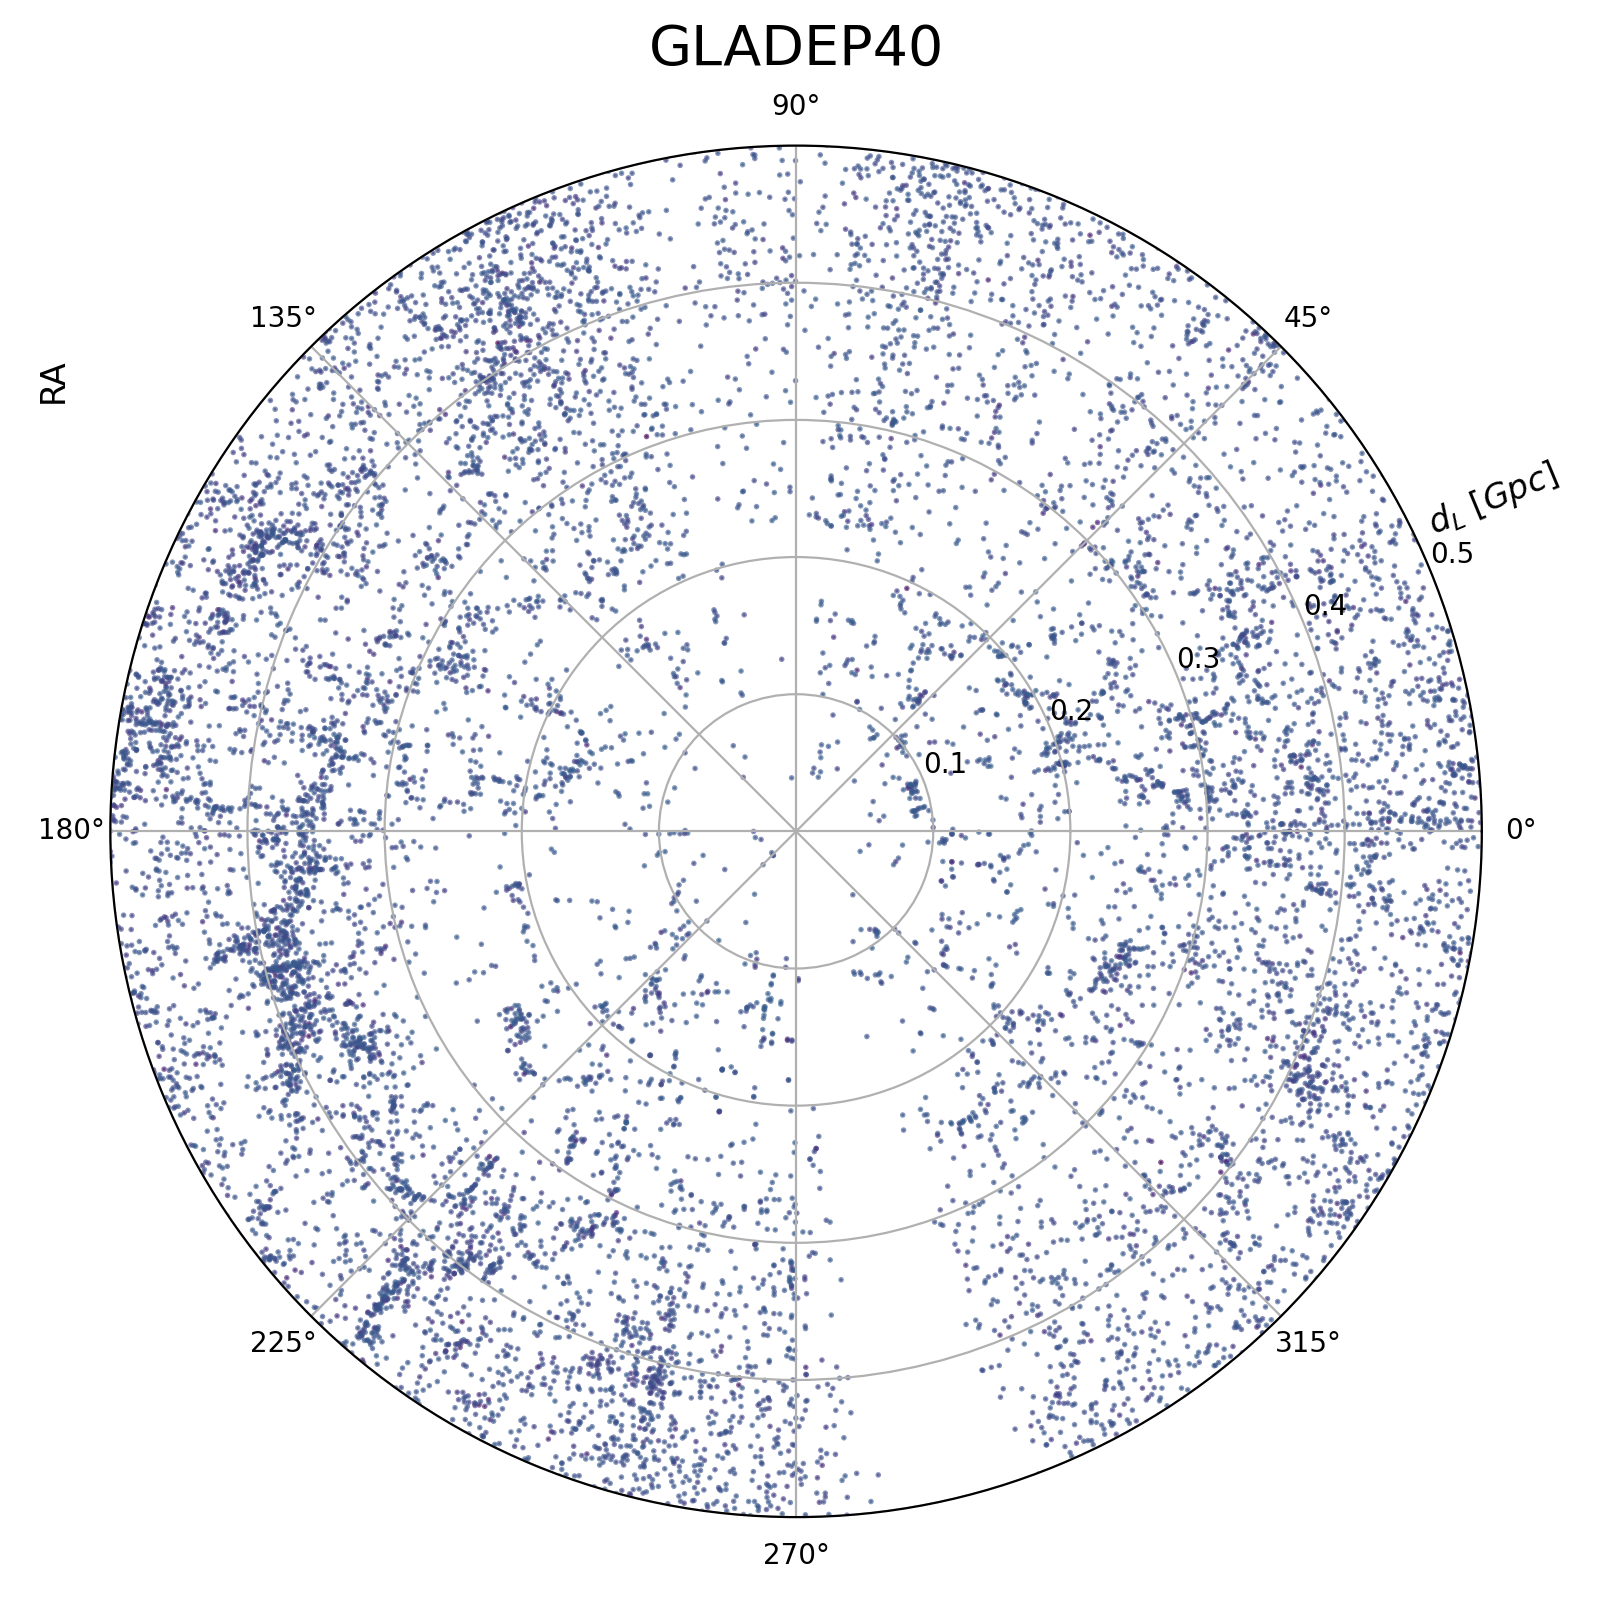
\includegraphics[width=\linewidth]{figures/test_frame_g_6.png}
    \label{fig:gladep40}
  \end{subfigure}
  \begin{subfigure}{0.32\textwidth}
    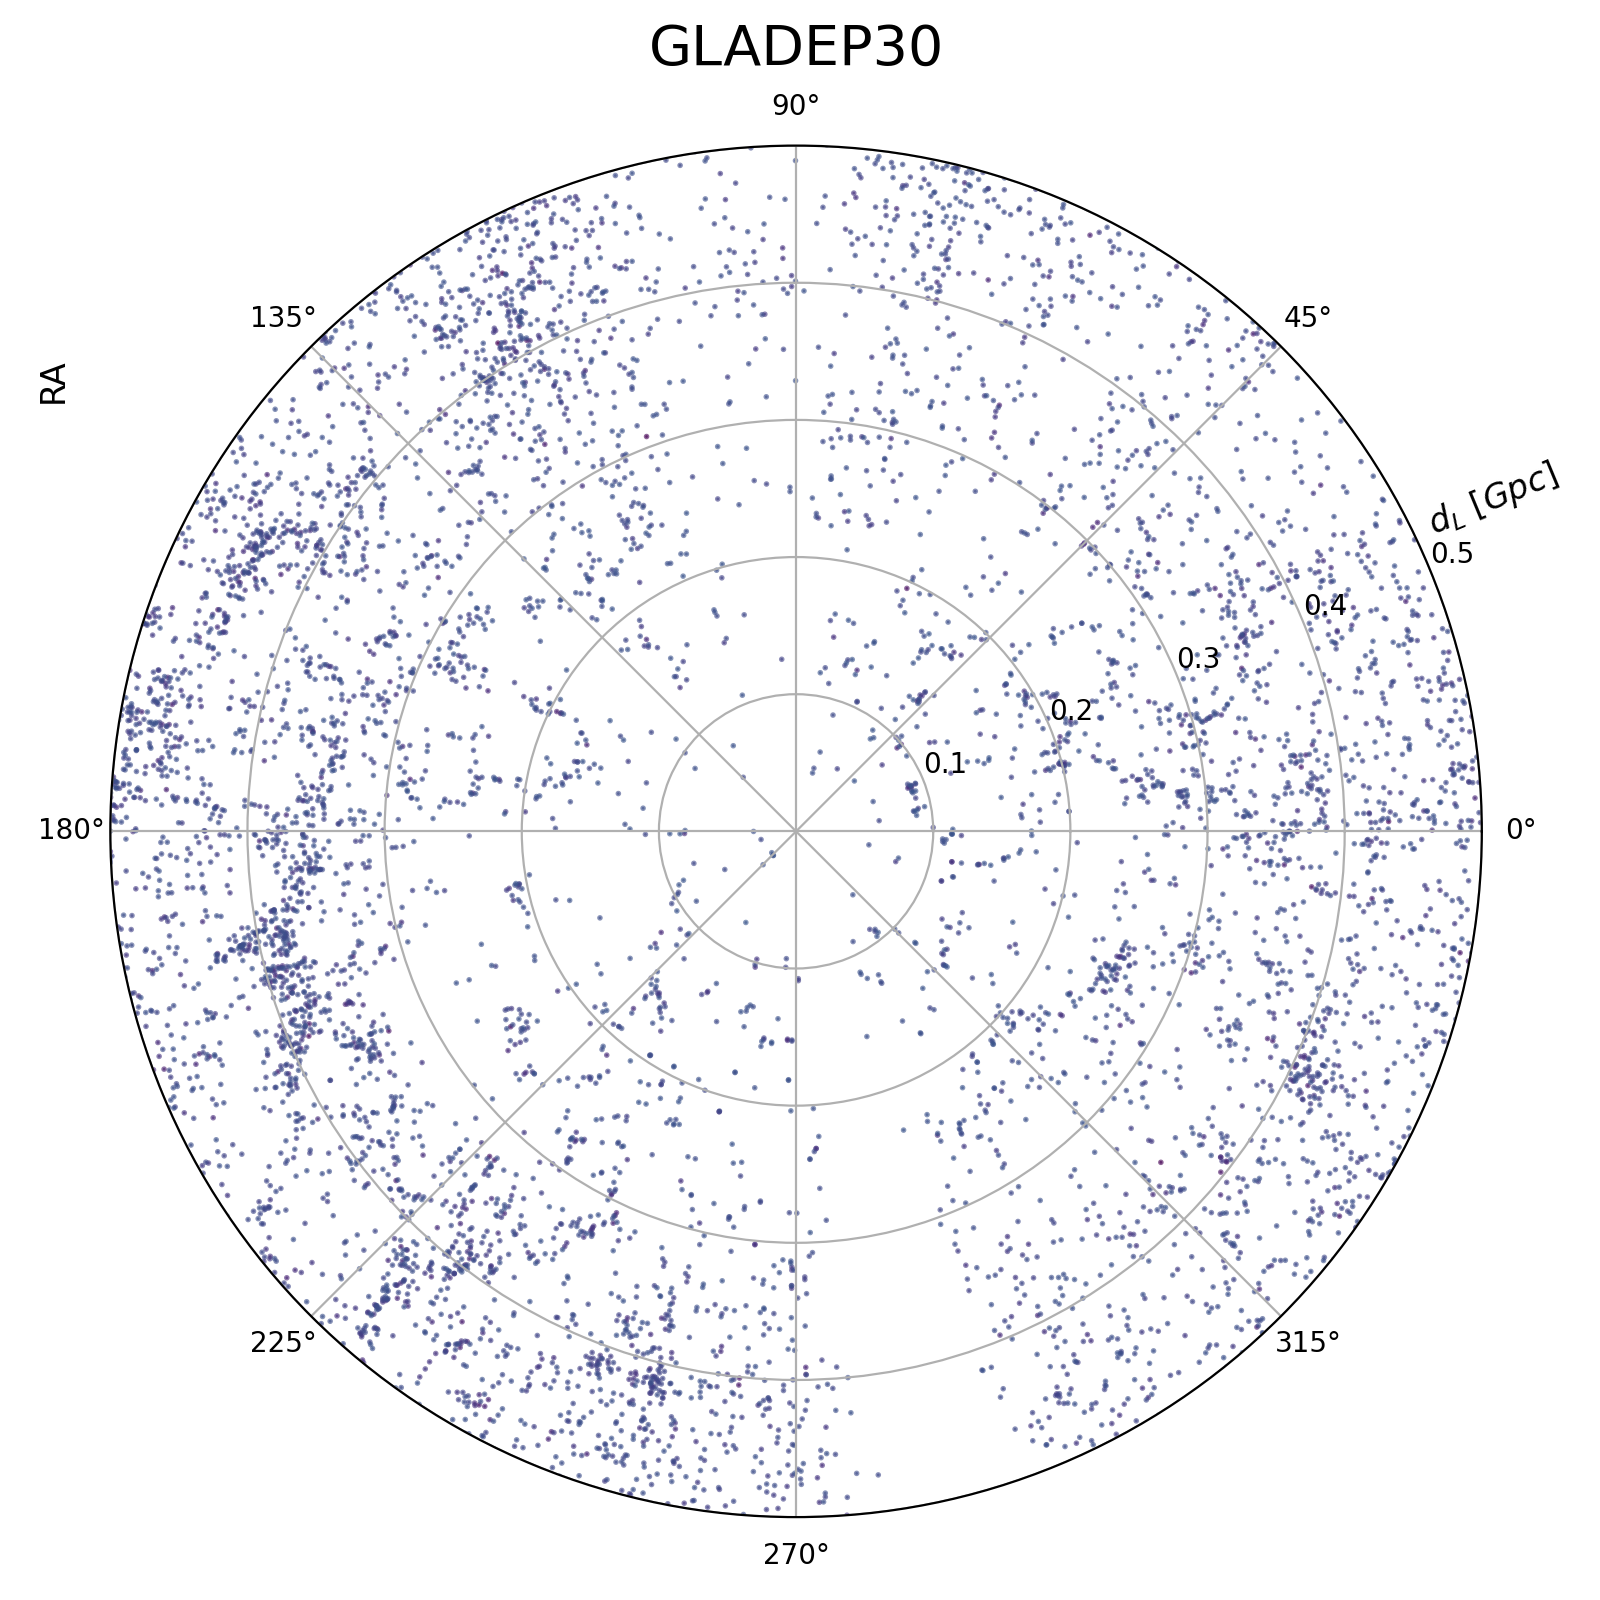
\includegraphics[width=\linewidth]{figures/test_frame_g_7.png}
    \label{fig:gladep30}
  \end{subfigure}
  \begin{subfigure}{0.32\textwidth}
    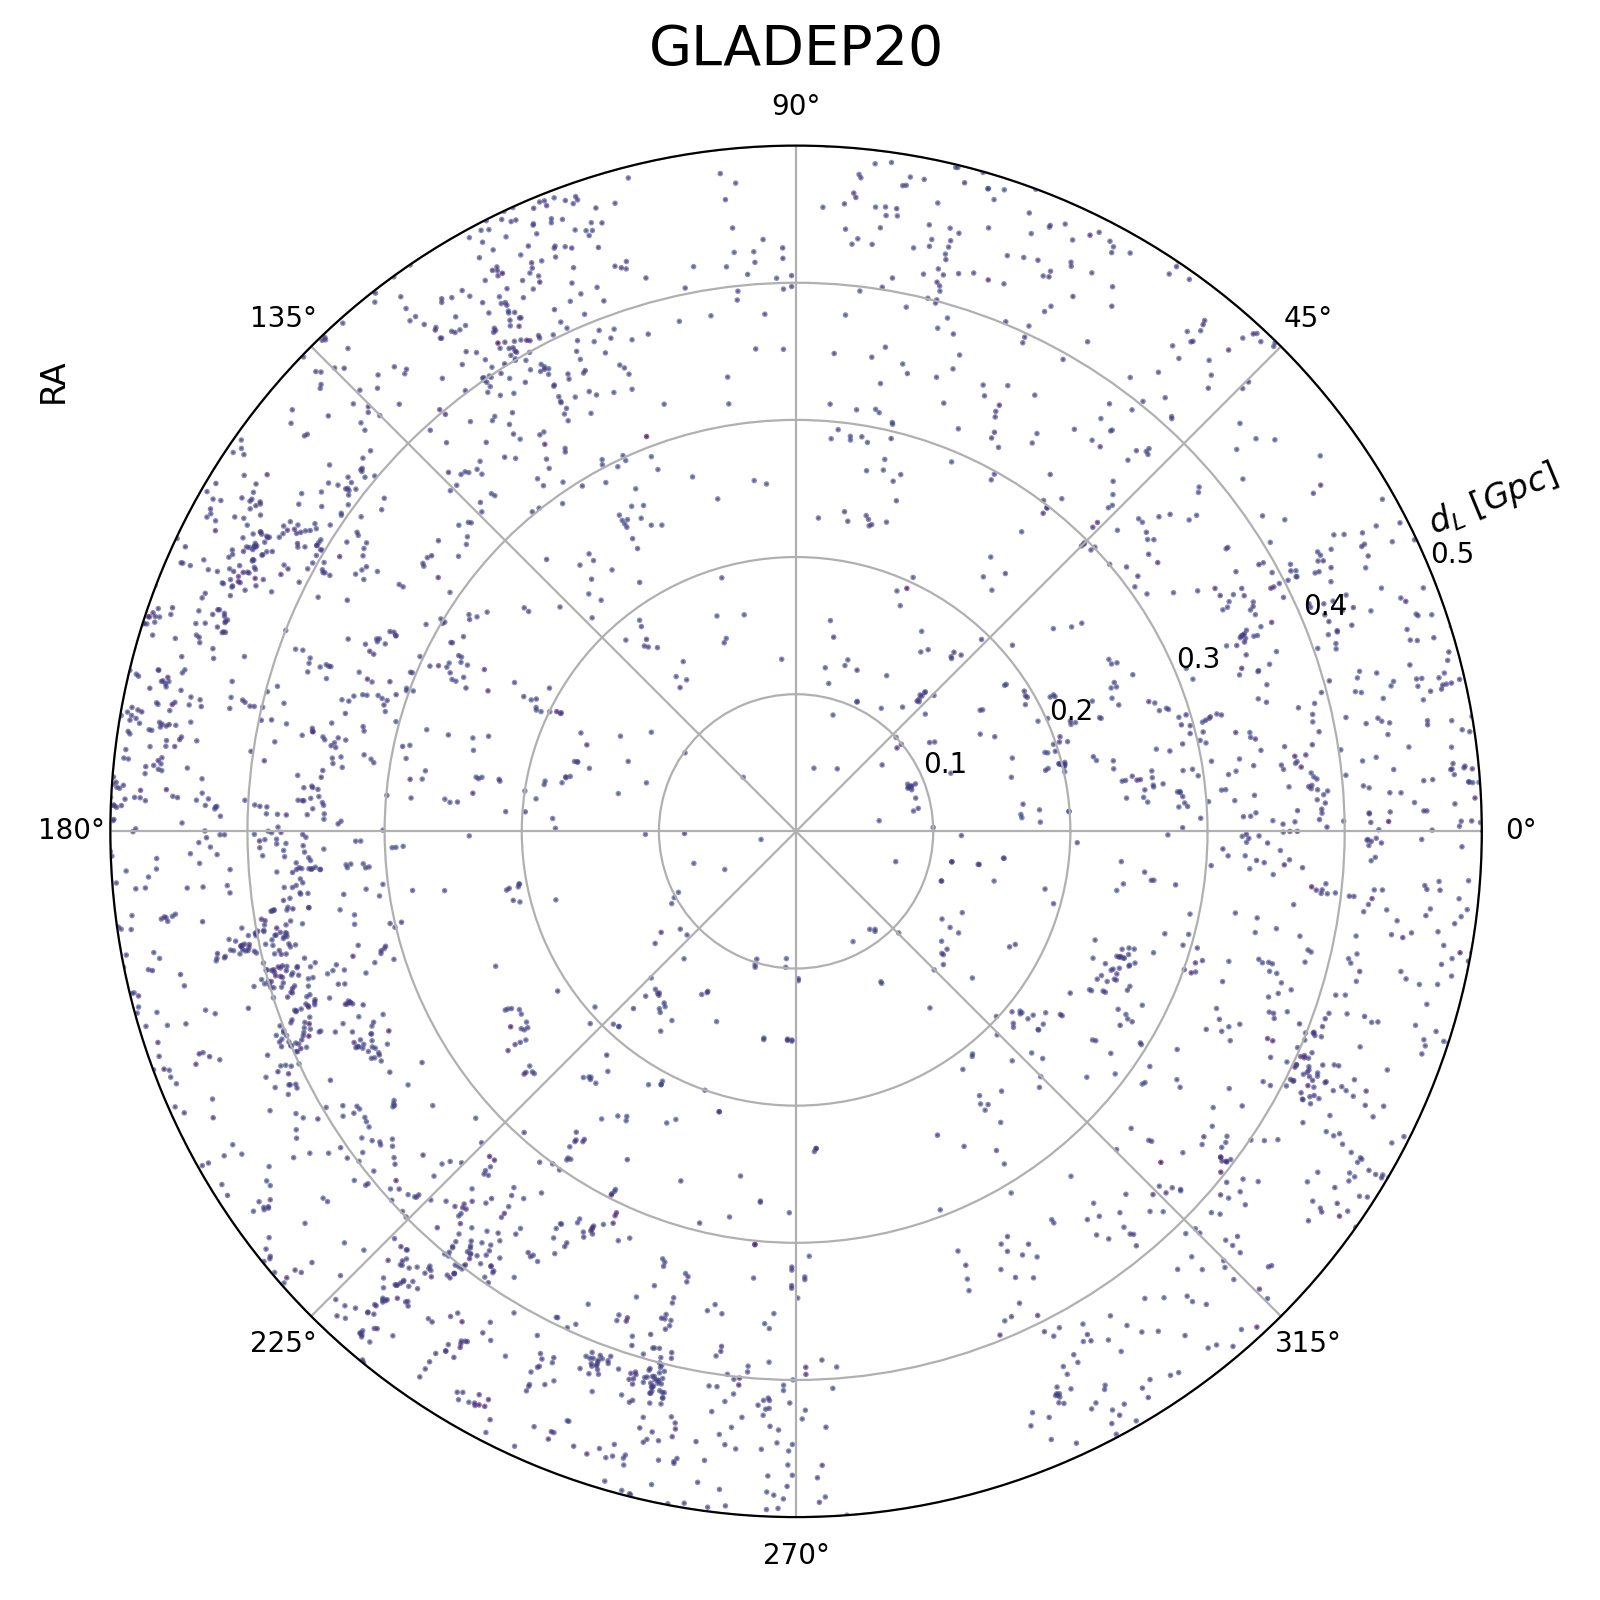
\includegraphics[width=\linewidth]{figures/test_frame_g_8.png}
    \label{fig:gladep20}
  \end{subfigure}

  \vspace{0.5em}

  \begin{subfigure}{0.32\textwidth}
    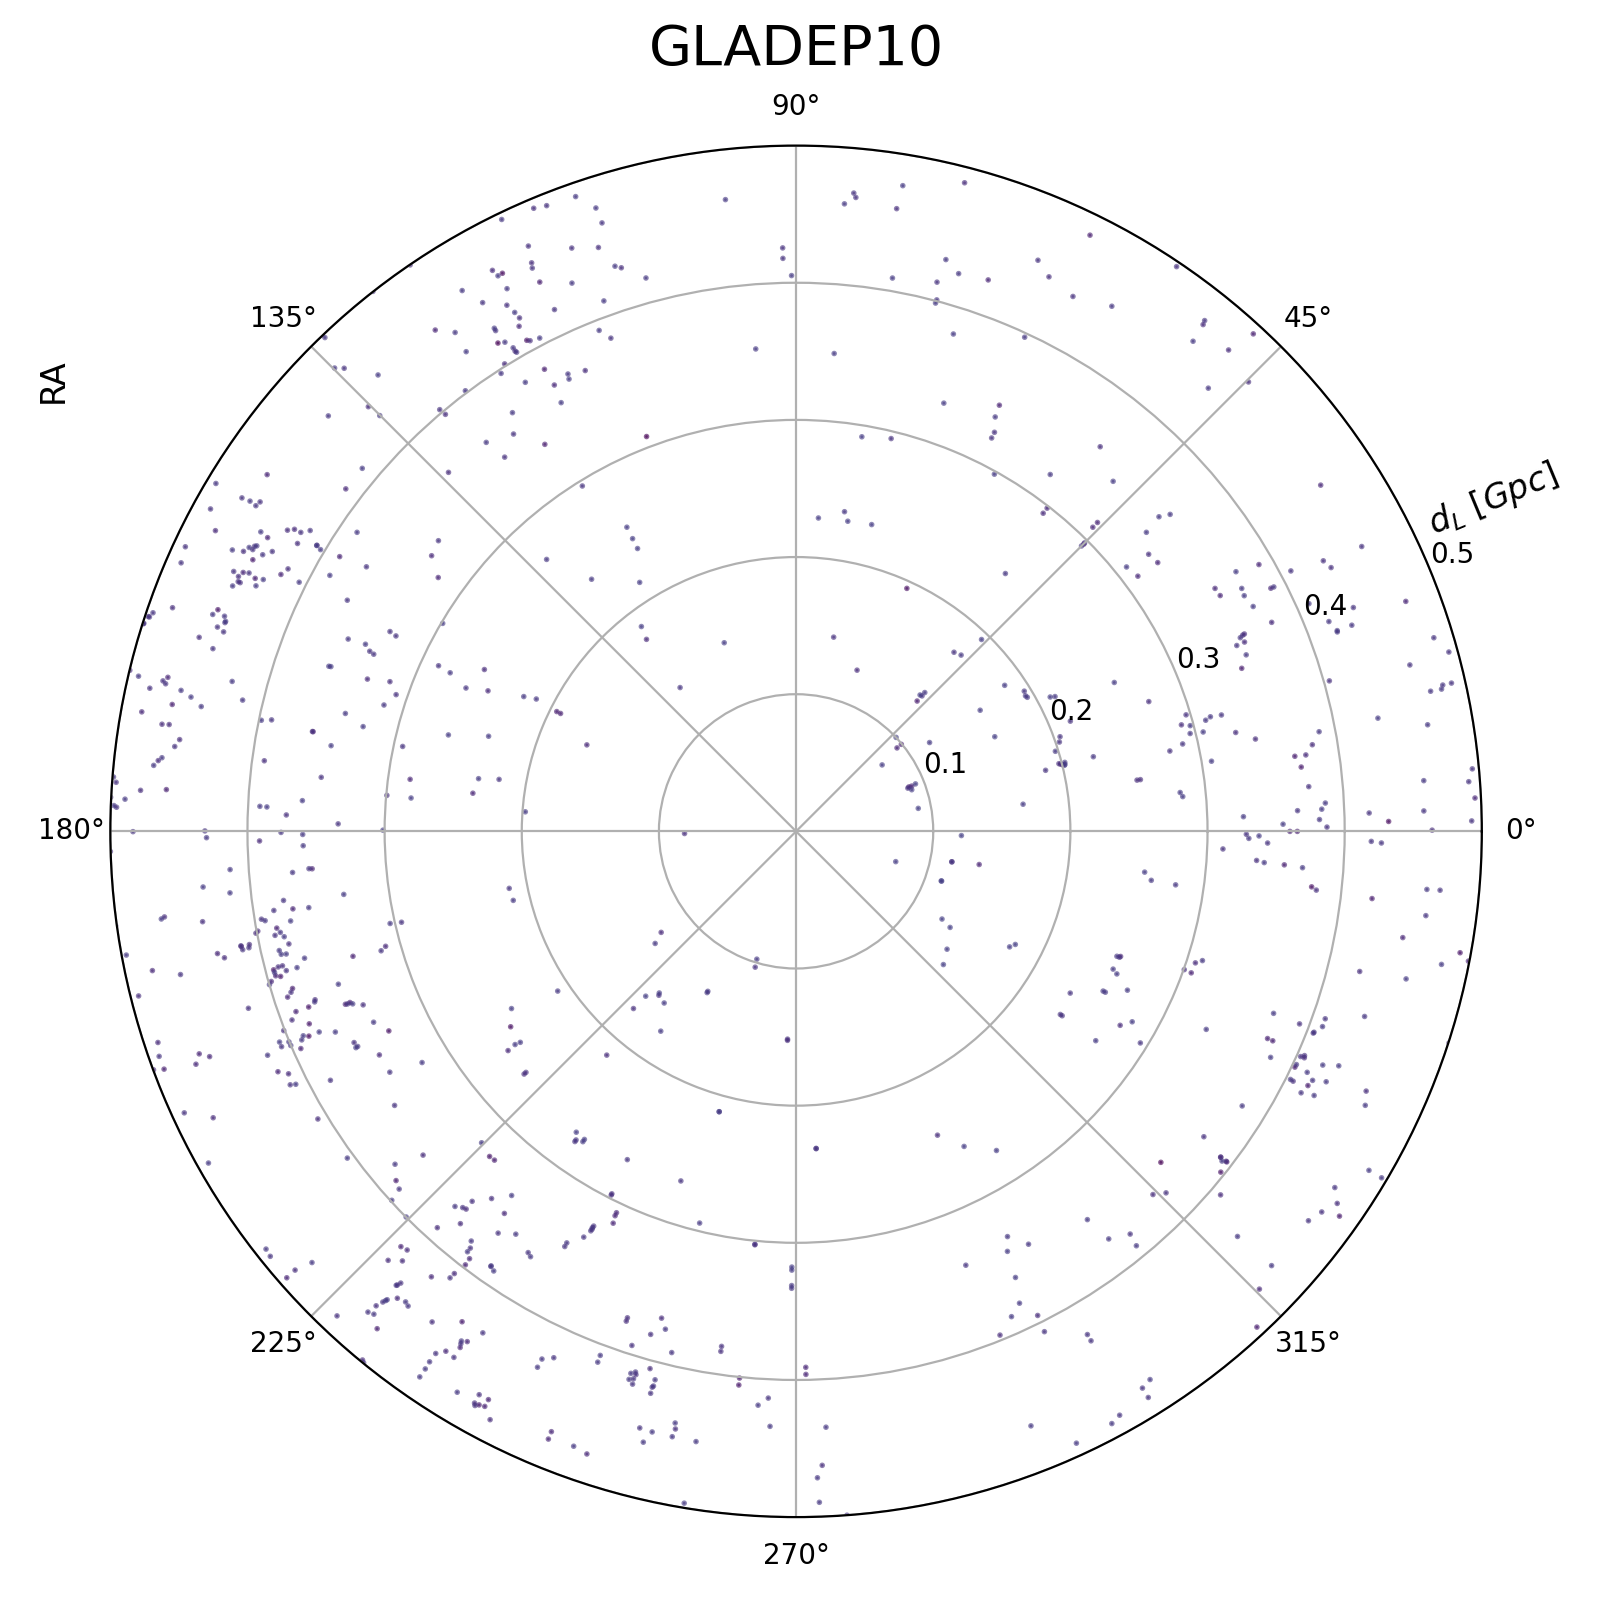
\includegraphics[width=\linewidth]{figures/test_frame_g_9.png}
    \label{fig:gladep10}
  \end{subfigure}
  \begin{subfigure}{0.64\textwidth}
    \centering
    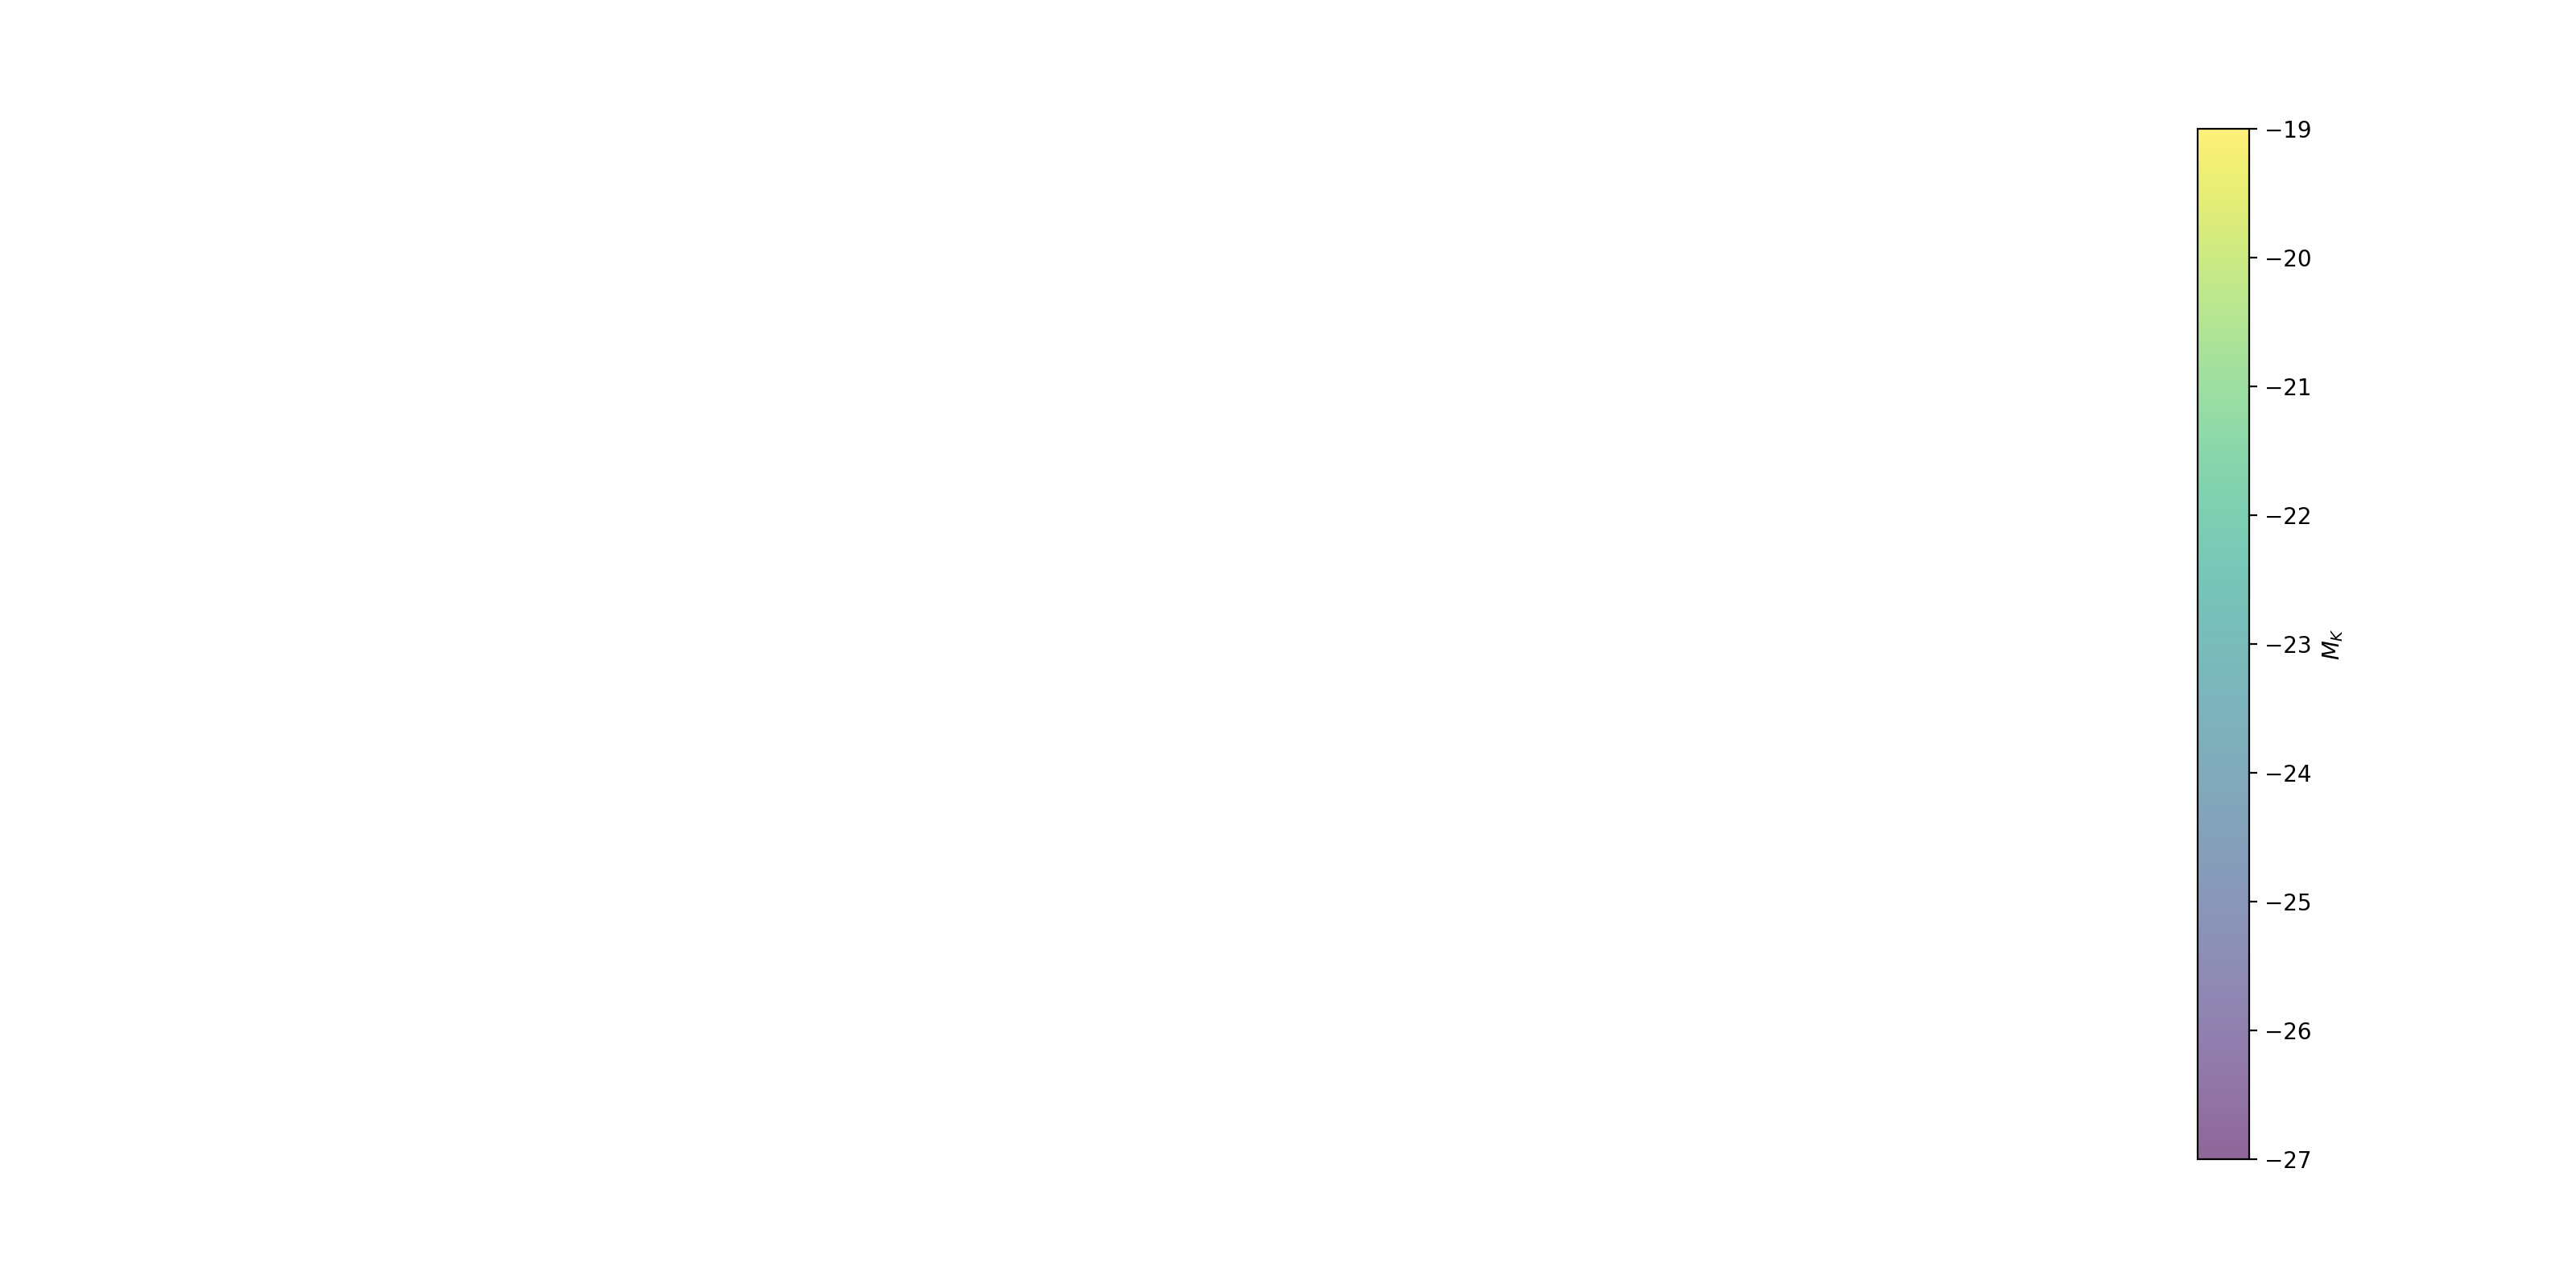
\includegraphics[width=\linewidth]{figures/test_frame_g_colorbar.png}
    \vspace{0.02em}
  \end{subfigure}

  \caption[Spatial distribution of galaxies from the GLADE+ galaxy catalog and its subsets.]{Spatial distribution of galaxies from the GLADE+ catalog and its bright subsets, employed for dark standard siren cosmology. The plots show a 10-degree slice in declination, centered at $0^\circ$, with the radial coordinate representing luminosity distance $d_L$ (in Gpc) and the angular coordinates being right ascension (RA). This shows how the bright galaxies trace the large-scale structure of the Universe.}
  \label{fig:dist_gladep}
\end{figure}


\newpage

\section{\Ac{LOS} Redshift Prior}
%We base our analysis on the \texttt{gwcosmo} pipeline \citep{gray2020cosmological,gray2022pixelated,gray2023joint}, which relies on a precomputed \ac{LOS} redshift prior, a prior on the \ac{GW} signal's redshift and direction. This \ac{LOS} redshift prior is used in tandem with the luminosity distance posterior from the \ac{GW} signal, to get a measurement for the Hubble constant $H_0$.

As \texttt{gwcosmo} requires a redshift prior for each \ac{GW} event, we construct a \ac{LOS} redshift prior from the \texttt{GLADE+} galaxy catalog. The \texttt{GLADE+} catalog is a comprehensive database of galaxies in the local Universe, which provides information about their positions, redshifts, and luminosities. This catalog is used to construct a redshift prior for each \ac{GW} event, which is used in tandem with the luminosity distance posterior from the \ac{GW} signal, to get a measurement for the Hubble constant $H_0$.

\subsection{\ac{LOS} Redshift Prior Construction}
The \ac{LOS} redshift prior is constructed from the \texttt{GLADE+} galaxy catalog, which contains a wealth of information about the galaxies in the local Universe. The redshift prior is constructed by taking into account the distribution of galaxies along the line of sight to the \ac{GW} event, as well as their luminosity and redshift. This allows us to obtain a more accurate estimate for the redshift of the \ac{GW} signal, which is crucial for cosmological measurements. The prior is constructed by dividing the sky into HEALPix pixels, and computing the redshift distribution of galaxies in each pixel. The redshift prior is then weighted using the luminosity of the potential host galaxies, allowing us to obtain a more accurate estimate for the Hubble constant.

Furthermore, the prior accounts for the incompleteness of the galaxy catalog, using source population models and the magnitude threshold calculated per pixel, which is particularly important for high-redshift events where the number of galaxies is significantly reduced. This allows us to separate the \ac{LOS} redshift prior into an in-catalog and out-of-catalog contribution.

Taking into account, the fact that the host galaxy can be present, or not, inside the catalog, one can write the \ac{LOS} redshift prior as:
\begin{align}
  p(z|\Omega_i, \Lambda, s, I) =& \iint \sum_{g=G,\bar{G}} p(z, M, m,g|\Omega_i, \Lambda, s, I)~dM dm \\
  =&~p(G|\Omega_i, \Lambda, s, I) \iint p(z, M, m|G,\Omega_i, \Lambda, s, I)~dM dm \nonumber \\
  &+ p(\bar{G}|\Omega_i, \Lambda, s, I) \iint p(z, M, m|\bar{G},\Omega_i, \Lambda, s, I)~dM dm
\end{align}

The first term in the equation represents the contribution from galaxies that are present in the catalog, while the second term represents the contribution from galaxies outside the catalog. The two terms are weighted by their respective probabilities of being present or not in the catalog. The terms inside the integral are the priors on the redshift $z$, absolute magnitude $M$, and apparent magnitude of the galaxies $m$, informed by the galaxy catalog, within the sky area covered by pixel $i$. Here the parameters $G/\bar{G}$ give the presence or absence of the galaxy in the catalog, $\Omega_i$ the sky location of the \ac{GW} event, $\Lambda$ the cosmological and population hyperparameters of interest, $s$ the presence of a \ac{GW} source, and $I$ the additional assumptions which are not excplicitly expressed. One also needs to marginalize over the absolute magnitude $M$ and the apparent magnitude $m$ of the galaxy, as these determine, to the leading order, which galaxiess are present in a flux-limited \ac{EM} survey \citep{gray2023joint}.

%\subsubsection{In-Catalog Contribution}
The integral in the in-catalog term can be expressed as the sum over the possible host galaxies in the catalog, weighted by their respective probabilities of being the host galaxy. These galaxies are weighted by their luminosity, which is a function of the absolute magnitude and redshift. The rationale being that the more luminous, and thus heavier galaxies are more likely to host \ac{CBC} events, and therefore contribute more to the \ac{LOS} redshift prior. This reduces the in-catalog part to a wieghted sum over the galaxies in the catalog, where the galaxies are treated as point sources modeled by a Gaussian. This term can thus be expressed as:
\begin{align}
  \iint p(z, M, m|G,\Omega_i, \Lambda, s, I)~dM dm =& \frac{1}{p(s|G,\Omega_i, \Lambda, I)N_{\mathrm{gal}}(\Omega_i)} \nonumber\\ 
  &\times \sum_{k}^{N_{\mathrm{gal}}(\Omega_i)} p(z|\hat{z}_k) p(s|z, M(z, \hat{m}_k, \Lambda), \Lambda, I)
\end{align}
where the term $p(z|\hat{z}_k)$ represents the probability of a galaxy being at redshift $z$, given its observed redshift $\hat{z}_k$. This term is used to weight the contribution from each galaxy in the catalog, based on its observed redshift.

%\subsubsection{Out-of-Catalog Contribution}
The integral in the out-of-catalog term marginalizes over the possible host galaxies not present in the catalog. This term is more complex, as it requires a model for the distribution of galaxies in the Universe, which is not directly available from the catalog. We use a Schechter luminosity function to model the distribution of galaxies in the Universe, which allows us to estimate the contribution from galaxies outside the catalog. The out-of-catalog term can be expressed as:
\begin{align}
  \iint & p(z, M, m|\bar{G},\Omega_i, \Lambda, s, I)~dM dm \nonumber \\
  &= \frac{1}{p(s|\bar{G},\Omega_i, \Lambda, I)p(\bar{G}|\Omega_i, \Lambda, I)} \nonumber \\ 
  &~~~\times \Bigg[\Theta[z_{\mathrm{cut}} -z] \int_{M(z,m_{\mathrm{thr}}(\Omega_i), \Lambda)}^{M_{\mathrm{max}}(H_0)} p(z,M|\Lambda, I) p(s|z,M,\Lambda,I)~dM \nonumber \\
  &\qquad \quad + \Theta[z-z_{\mathrm{cut}}] \int_{M_{\mathrm{min}}(H_0)}^{M_{\mathrm{max}}(H_0)} p(z,M|\Lambda, I) p(s|z,M,\Lambda,I)~dM \Bigg]
\end{align}
Here we also account for the \ac{EM} selection effects of the catalog. Due to the flux limited nature of the galaxy catalog, the probability of a galaxy being present in the catalog depends on the galaxy's apparent magnitude, and whether it is greater or smaller than apparent magnitude threshold of the catalog along the same line of sight, $m_{\mathrm{th}}(\Omega_i)$. The Heaviside function $\Theta$ is used to separate the two cases of the out-of-catalog contribution, depending on whether the redshift $z$ is below or above a certain threshold $z_{\mathrm{cut}}$. This is due to to the exclusion of galaxies with redshift $z$ greater than $z_{\mathrm{cut}}$ from the catalog, which is a result of unreliable redshift or color information at these higher redshifts.

The term $p(s|z,M,\Lambda,I)$ is the weighting factor for the contribution from each galaxy, based on its luminosity and redshift. The galaxies are weighted by their luminosity in the $K$-band, which is a good tracer of the mass of the galaxies \citep{strazzullo2006near,sureshkumar2021galaxy}. Furthermore, the merger host probability is also taken into account, which is a function of the redshift. This is modeled by a Madau-Dickinson merger rate evolution model \citep{madau2014cosmic}, which describes the evolution of the merger rate with redshift, discussed in Section \ref{sec:source_population}. The term $p(s|z,M,\Lambda,I)$, also incorporates the source population models, used to populate the out-of-catalog contribution. These models are also discussed in Section \ref{sec:source_population}.

The term $p(z,M|\Lambda, I)$ represents the luminosity funtion of the galaxies, taken to be the Schechter luminosity function, discussed in Section \ref{sec:luminosity_function}. The integration limits are set by the minimum and maximum absolute magnitudes of the galaxies, $M_{\mathrm{min}}(H_0)$ and $M_{\mathrm{max}}(H_0)$. These are $H_0$-dependent, as the parameters of the Schechter luminosity function are also $H_0$-dependent, but the final distribution remains insensitive to the exact values of $H_0$ \citep{gray2023joint}.

\section{Results}
In this section we present the main outcomes of our analysis: how applying brightness cuts to the \texttt{GLADE+} catalog alters \ac{LOS} redshift prior for individual events, how these modified priors propagate into the inferred posterior on the Hubble constant $H_0$. It should be noted that while \texttt{gwcosmo} is designed to perform joint population and cosmological inference, we focus here on the impact of the brightness cuts on the \ac{LOS} redshift prior and the resulting $H_0$ posterior. For this reason, we do not perform a full joint inference, but rather use \texttt{gwcosmo} for $H_0$ inference, while keeping the population hyperparameters fixed to the values mentioned in Section~\ref{sec:source_population}.

To test the impact of catalog completeness, we apply successive cuts to the galaxy catalog by selecting only the brightest $XX\%$ of galaxies in $K$-band luminosity, forming subsets labeled \texttt{GLADEPXX}. This process shifts the effective redshift upwards, reducing the number of galaxies but improving the catalog's completeness.

\subsection{\ac{LOS} Redshift Prior}
Figure~\ref{fig:los_prior_gw170809} shows the LOS redshift prior for the event \textbf{GW170809} under different catalog cuts. Bright galaxy subsets (e.g., \texttt{GLADEP20}) result in sharper redshift distributions and reduce the weight of the out-of-catalog term. The low-$z$ tail contributed by faint galaxies in the nearby Universe is also suppressed. Notably, these priors maintain consistency in shape, indicating that bright galaxies are reliable tracers of large-scale structure. The application of a brightness cut significantly modifies the \ac{LOS} redshift distribution. Specifically, the bright galaxy subsets yield an amplified redshift prior at higher distances, effectively extending the reach of the catalogue, somewhat mitigating the incompleteness issues that arise at deeper redshifts. This behavior is qualitatively consistent across events.

\begin{figure}[ht]
  \centering
  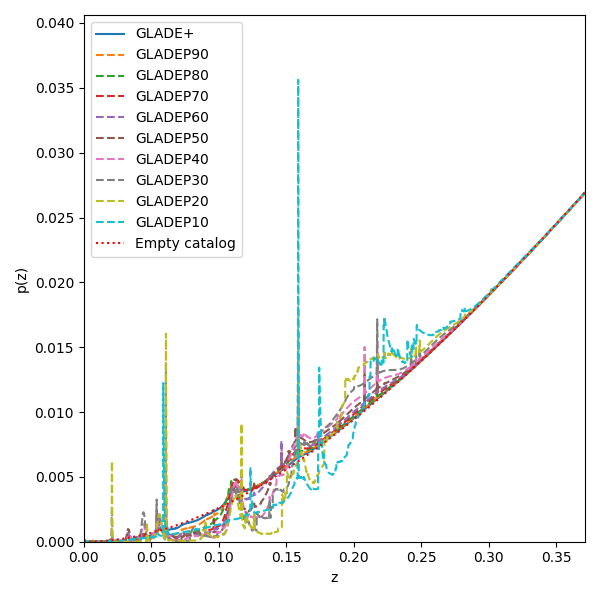
\includegraphics[width=0.67\textwidth]{figures/GW170809_zprior.png}
  \caption[LOS redshift prior for GW170809 for different brightness-ranked \texttt{GLADE+} subsets]{LOS redshift prior for GW170809 for different brightness-ranked \texttt{GLADE+} subsets. The full \texttt{GLADE+} catalog (solid blue) is compared to the different subsets. Applying a brightness cut amplifies the prior at higher distances, extending the effective reach of the catalog and partially mitigating incompleteness at greater redshifts.}
  \label{fig:los_prior_gw170809}
\end{figure}

\begin{figure}[h!]
  \centering
  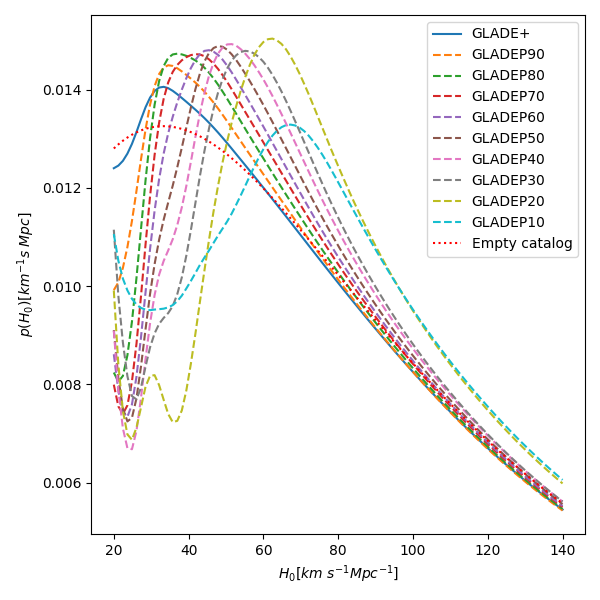
\includegraphics[width=0.67\textwidth]{figures/GW170809_H0.png}
  \caption[$H_0$ posterior distributions for GW170809 using different brightness-ranked \texttt{GLADE+} subsets.]{$H_0$ posterior distributions for GW170809 using different brightness-ranked \texttt{GLADE+} subsets. \texttt{GLADEP20} yields the tightest credible interval. \texttt{GLADEP10} suffers from sparse sampling.}
  \label{fig:h0_gw170809}
\end{figure}

\newpage

\subsection{Hubble Constant Posterior}

\begin{figure}[h!]
    \centering
    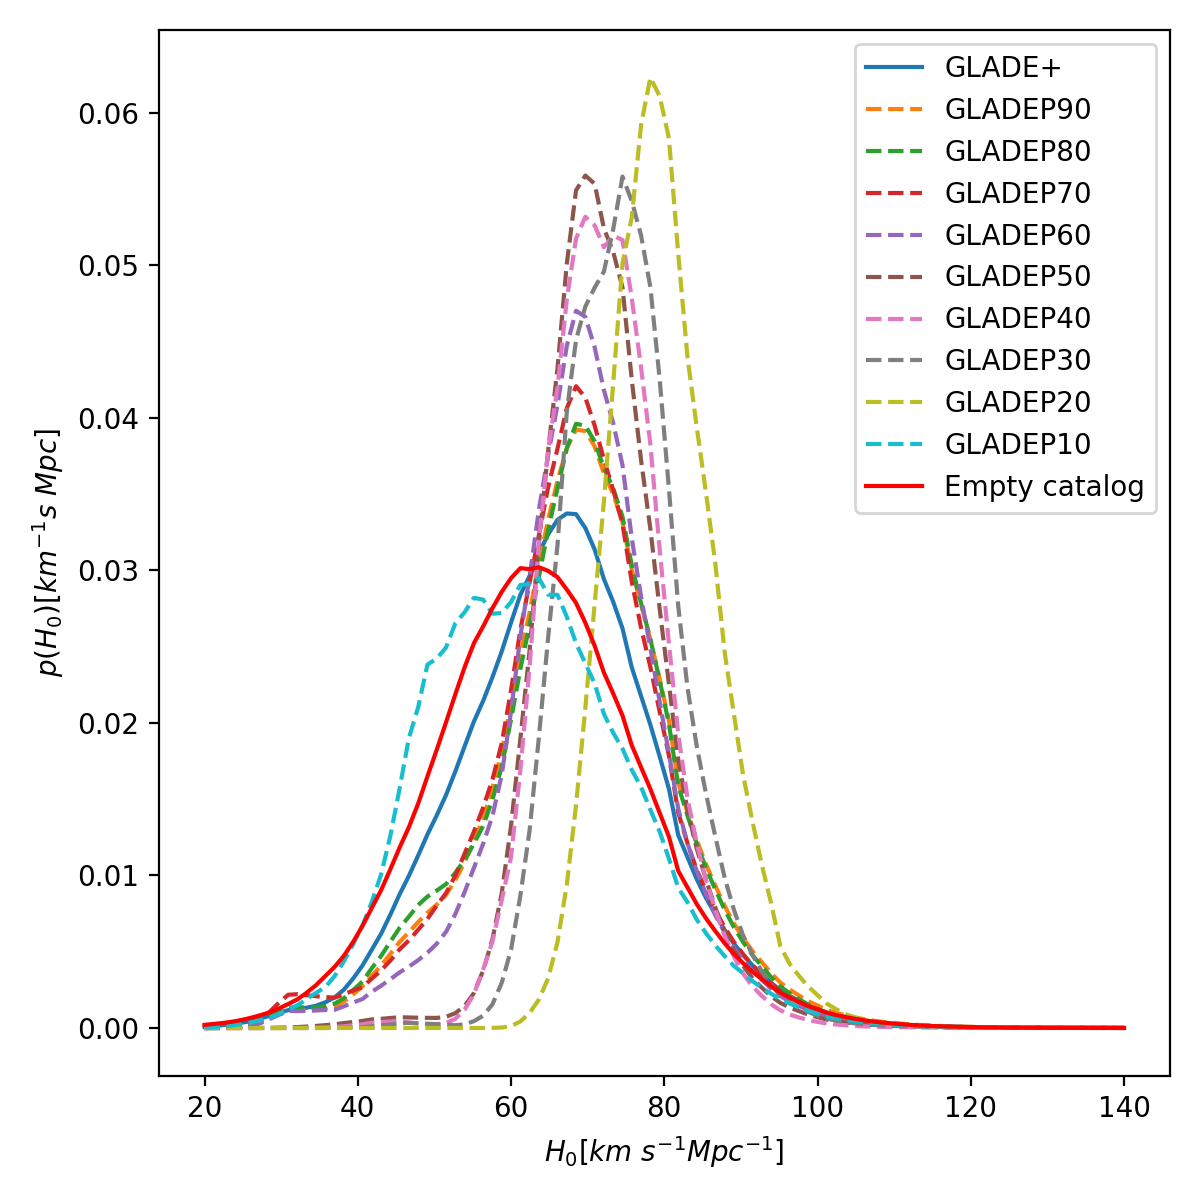
\includegraphics[width=0.67\textwidth]{figures/percentile_full_dict.png}
    \caption[Cumulative $H_0$ posterior from the selected dark siren events using full \texttt{GLADE+} and the different subsets.]{Cumulative $H_0$ posterior from the selected dark siren events using full \texttt{GLADE+} (blue) and the different subsets (dashed lines). The brightness-weighted catalog yields a tighter constraint without a significant shift.}
    \label{fig:h0_cumulative}
\end{figure}

\begin{table}
    \small
    \centering
    \caption[$H_0$ MAP values with $68\%$ confidence ranges, alongside the maximum magnitude limits for \texttt{GLADE+} and the different subsets.]{Maximum {\em a posteriori} probabilities with $68\%$ confidence ranges of the $H_0$ posterior distributions alongside the maximum magnitude limits for the different percentiles of the \texttt{GLADE+} galaxy catalogue.}
    \begin{tabular}{c c c }
    \hline
        \textbf{Catalogue} & $M_{K,\mathrm{max}}$ & $H_0~[\mathrm{km}~\mathrm{s}^{-1}\mathrm{Mpc}^{-1}]$ \\ \hline
        \\[-0.8em]
        \texttt{GLADE+} & $-19.00$ & $67.87^{+8.97}_{-10.29}$ \\ 
        \\[-0.8em]
        \texttt{GLADEP90} & $-23.07$ & $68.94^{+9.24}_{-7.55}$ \\
        \\[-0.8em]
        \texttt{GLADEP80} & $-23.62$ & $68.93^{+9.25}_{-7.57}$ \\
        \\[-0.8em]
        \texttt{GLADEP70} & $-23.94$ & $68.63^{+8.61}_{-7.42}$ \\
        \\[-0.8em]
        \texttt{GLADEP60} & $-24.19$ & $68.85^{+7.72}_{-6.43}$ \\
        \\[-0.8em]
        \texttt{GLADEP50} & $-24.14$ & $70.05^{+6.12}_{-5.20}$ \\
        \\[-0.8em]
        \texttt{GLADEP40} & $-24.63$ & $69.94^{+7.46}_{-3.88}$ \\
        \\[-0.8em]
        \texttt{GLADEP30} & $-24.87$ & $74.70^{+4.69}_{-6.58}$ \\
        \\[-0.8em]
        \texttt{GLADEP20} & $-25.15$ & $78.28^{+5.53}_{-4.95}$ \\
        \\[-0.8em]
        \texttt{GLADEP10} & $-25.53$ & $63.46^{+6.39}_{-14.37}$ \\ 
        \\[-0.8em]
        \hline
    \end{tabular}
    \label{tab:h0_stats}
\end{table}

Once one has the \ac{LOS} redshift prior, one can use it to compute the posterior distribution of the Hubble constant $H_0$ given the \ac{GW} event data, as the relation between the redhsift $z$, luminosity distance $d_L$ and the Hubble constant $H_0$ is given by:
\begin{align}
  d_L = \frac{c(1+z)}{H_0} \int_0^z \frac{dz'}{\sqrt{(1+z')^3\Omega_m + \Omega_\Lambda}}
\end{align}
for a flat $\Lambda$CDM cosmology. At lower redshifts, this can be simplified to:
\begin{align}
  d_L \approx \frac{cz}{H_0}
\end{align}
Thus the \ac{LOS} redshift prior, $p(z|\Omega_i, \Lambda, s, I)$, and the luminosity distance posterior, $p(d_L,\Omega\mid\mathrm{GW})$, from the \ac{GW} event data can be combined to obtain the posterior distribution of $H_0$, which can then be used to obtain constraints on the value of $H_0$.

Figure~\ref{fig:h0_gw170809} shows the resulting $H_0$ posteriors for GW170809 under various catalog cuts. As the catalog is restricted to brighter galaxies, the $H_0$ posterior becomes increasingly narrow. For example, \texttt{GLADEP20} yields a visibly tighter posterior compared to the full \texttt{GLADE+}, with a shift in the median. However, the most aggressive cut (\texttt{GLADEP10}) introduces broader tails, likely due to insufficient galaxy sampling in the localization volume.

We repeat this procedure for a subset of \ac{CBC} events from \ac{GWTC}-3 that meet our selection criteria. Figure~\ref{fig:h0_cumulative} shows the combined $H_0$ posterior from the selected dark siren events using the full \texttt{GLADE+} catalog and the different subsets. Table~\ref{tab:h0_stats} summarizes the $H_0$ posteriors for all cuts. The uncertainty is minimized around the \texttt{GLADEP20} subset, showing 30-40\% tighter contraints, while median values shift towards a higher value. While these tighter constraints are promising, the shift in median values could indicate a systematic bias introduced by the brightness cuts. This is particularly evident for the most extreme cut (\texttt{GLADEP10}), which yield a significantly lower median $H_0$ value, likely due to under-sampling and loss of information about the large-scale structure. For less extreme cuts, the median values doesn't show a huge shift. This suggests that moderate brightness cuts could improve precision without introducing much systematic bias.

\subsection{Luminosity Retention}
An important consideration when applying brightness-based cuts to galaxy catalogs is understanding how much of the total luminosity is retained as a function of the chosen percentile cut. Figure~\ref{fig:luminosity_fraction} shows the cumulative fraction of total $K$-band luminosity retained when selecting the brightest $X\%$ of galaxies in the \texttt{GLADE+} catalog.

As the figure illustrates, the retained luminosity decreases rapidly when pruning the catalog based on brightness. At first glance, this might suggest that discarding the fainter galaxies results in the loss of a significant portion of cosmologically relevant information. However, this effect is largely driven by the overwhelming number of faint galaxies, each contributing only marginally to the total light output. 

It is also important to note that the selection is made using the brightest percentiles of the catalog itself, rather than a parametric cut based on a fitted Schechter function. This empirical approach includes all galaxies below a certain magnitude threshold, which accentuates the cumulative effect of the numerous low-luminosity galaxies and contributes to the pronounced loss observed in total luminosity.

\begin{figure}[h]
    \centering
    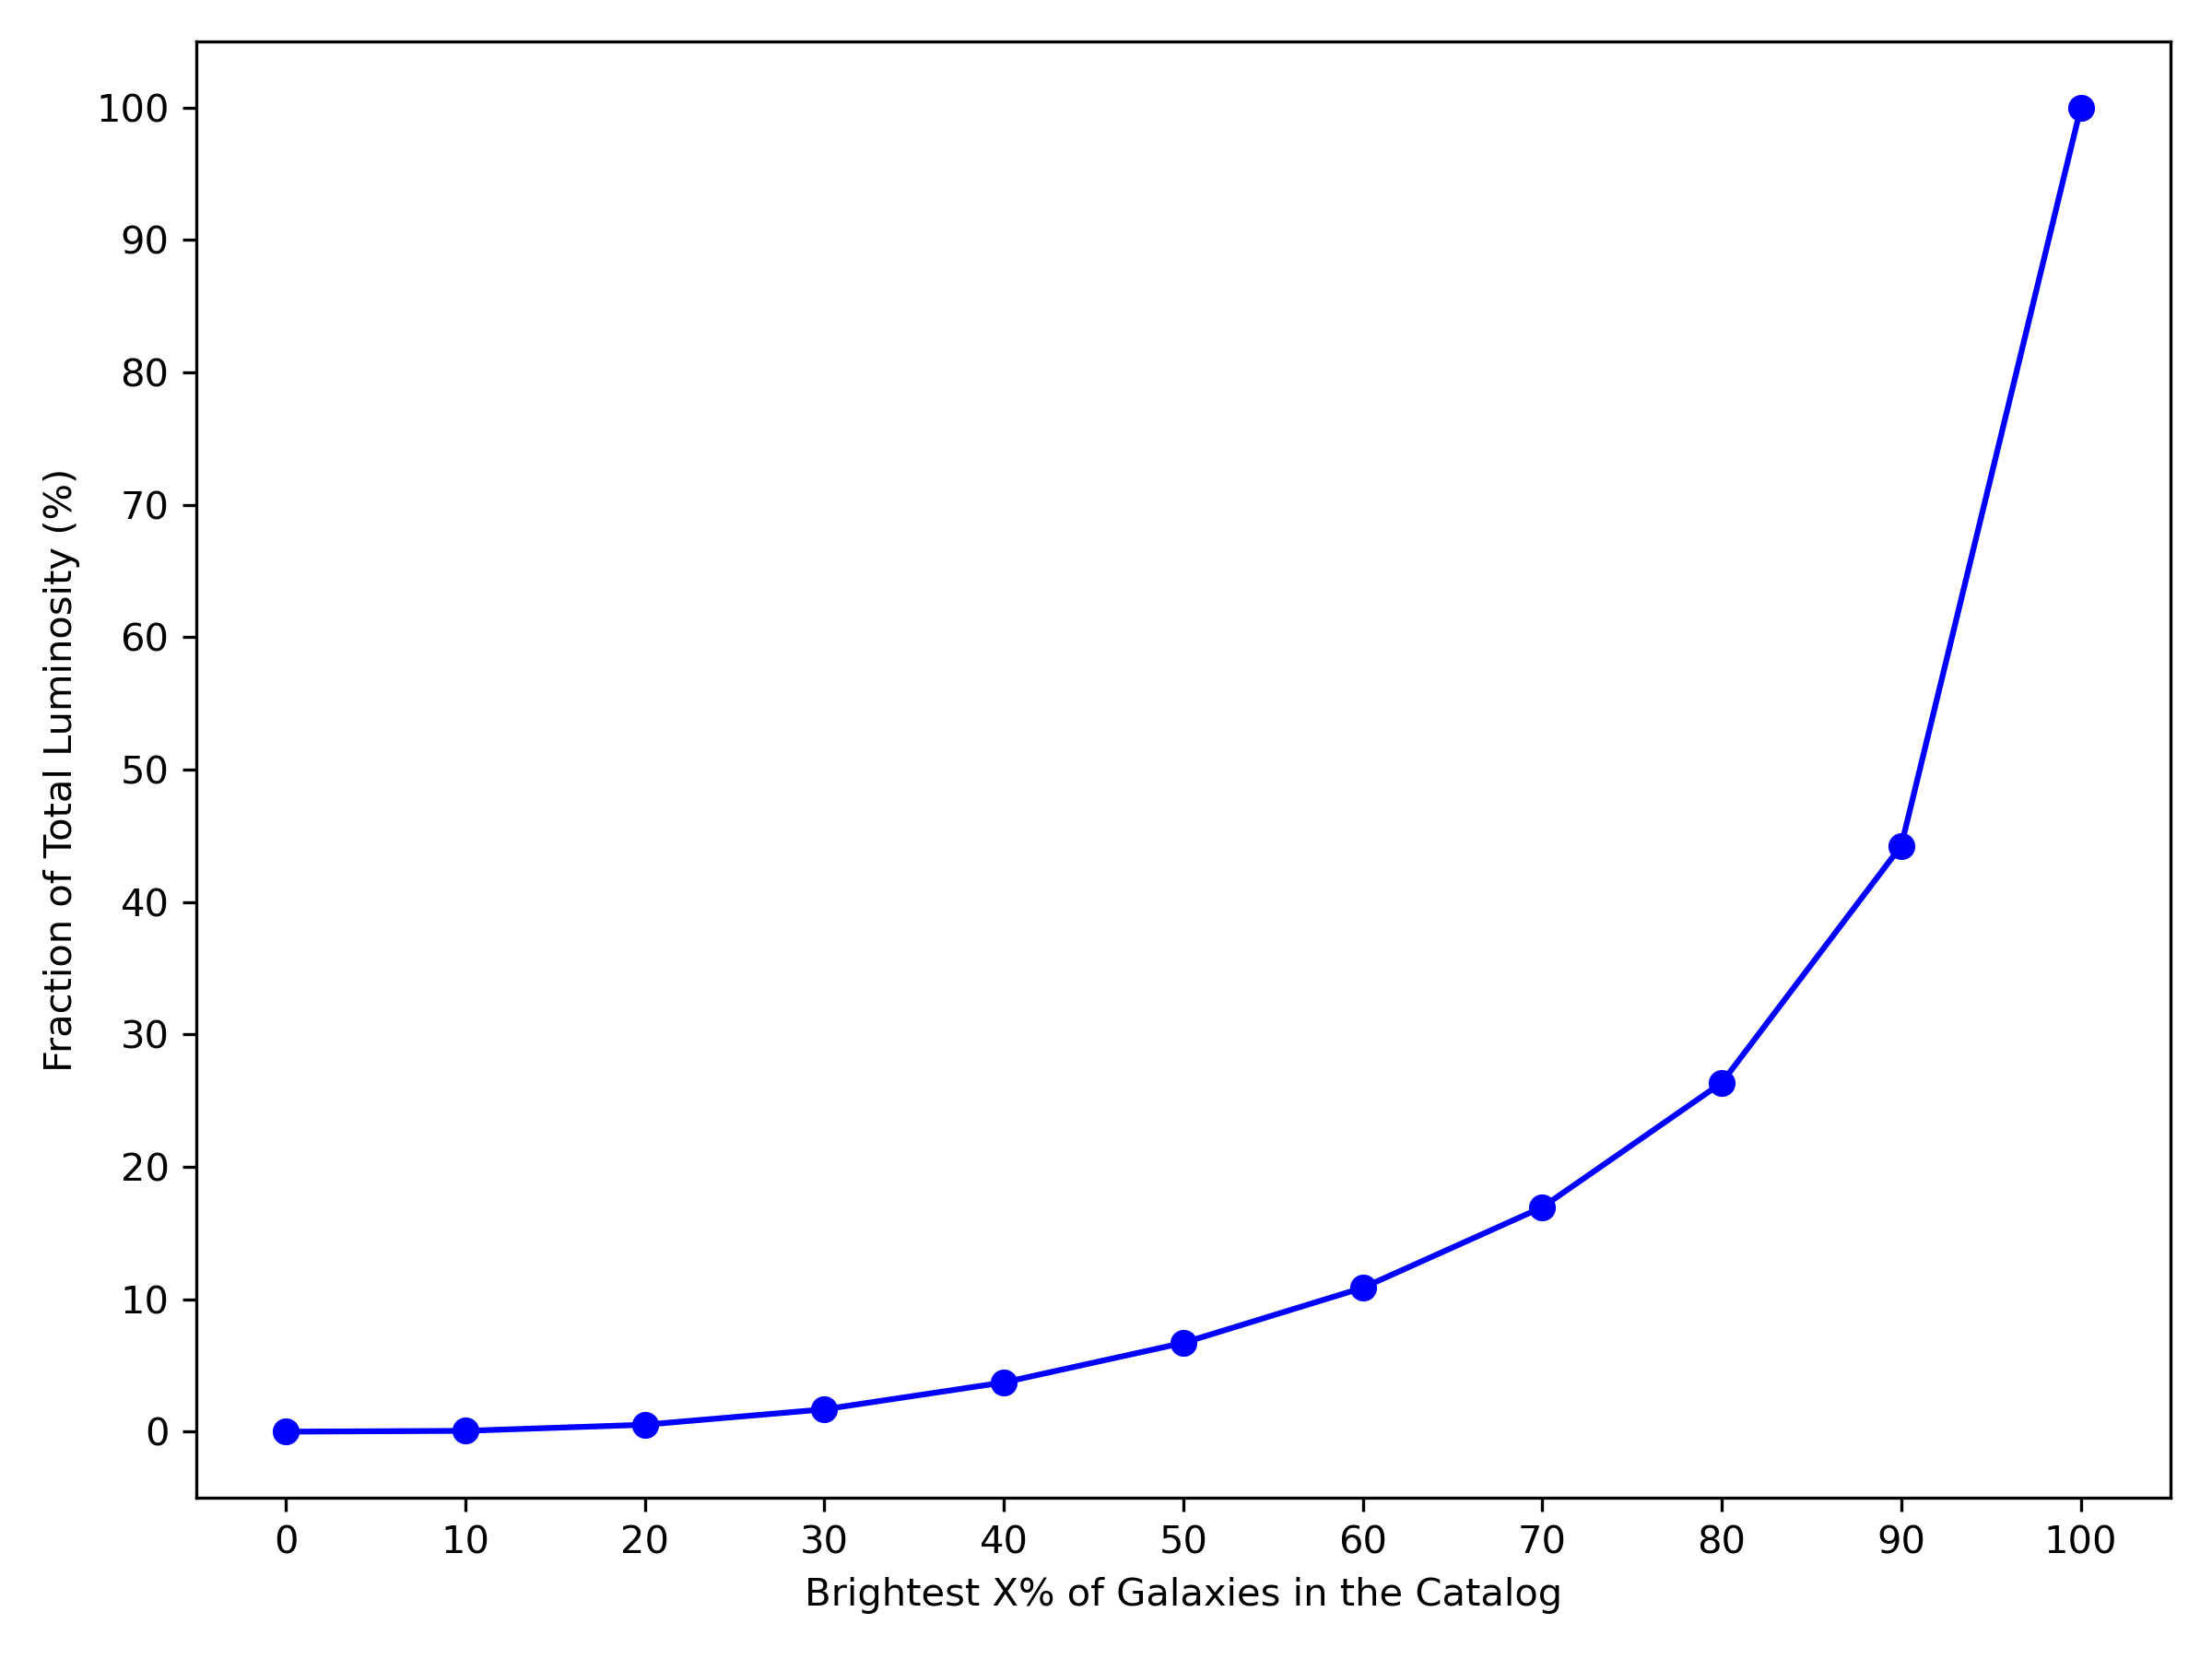
\includegraphics[width=0.7\textwidth]{figures/luminosity_fraction_vs_percentile_GLADE.png}
    \caption[\texttt{GLADE+} luminosity retention.]{Fraction of total $K$-band luminosity as a function of the brightest $X\%$ of galaxies in the catalog. The steep slope near 100\% reflects the contribution of the numerous dim galaxies to the total luminosity budget.\footnotemark}
    \label{fig:luminosity_fraction}
\end{figure}
\footnotetext{This plot was generated using code partially adapted from scripts provided by Cezary Turski.}

The bright galaxies we retain are intrinsically more luminous and are typically associated with massive halos and central locations in galaxy groups or clusters. These bright, high-mass galaxies are more likely to trace the underlying matter distribution, which is essential for our purpose. By focusing on the top percentiles in brightness, we sacrifice luminosity but preserve the most structurally informative objects.

Therefore, while the pruning strategy leads to a steep loss in integrated light (as shown in the figure), this primarily reflects the exclusion of numerous dim galaxies that do not significantly enhance the galaxy density field used to construct the redshift prior. The retained bright galaxies should still provide a robust tracer of large-scale structure, particularly at higher redshifts where catalog completeness begins to decline.

\subsection{Cost-Benefit Trade-Off}
We observe that the precision of the $H_0$ posterior improves as the catalog is pruned to include only the brightest galaxies, up to an optimal point (around \texttt{GLADEP20}). Beyond this point, the constraints begin to degrade, with the posterior broadening and approaching the result obtained with an empty catalog. This degradation arises from under-sampling the galaxy distribution, highlighting a practical limit to brightness-based pruning.

While brightness cuts can enhance statistical precision by removing noisy or weakly informative galaxies, they also risk excluding key structure-tracing galaxies if pushed too far. This trade-off between precision and completeness must be carefully managed, as overly aggressive cuts can introduce bias and weaken the reliability of cosmological inference. The exact location of the optimal cut may depend on the specifics of the GW event, such as its localization volume, and the characteristics of the underlying galaxy catalog.

This balance is best understood within the framework of the \acf{MDC}, which is discussed in the next chapter. The \ac{MDC} allows us to systematically test how different cuts affect the inferred $H_0$, providing a controlled environment to evaluate potential biases and performance.

Our results suggest that targeting the brightest galaxies in a well-characterized catalog can substantially enhance the precision of $H_0$ measurements from dark sirens. This method serves as a complementary approach to other strategies for mitigating catalog incompleteness, such as joint inference with galaxy clustering or population-based redshift estimation.